%HEADER:
\documentclass{article}
\usepackage[UTF8]{ctex}%Chinese supporting
\usepackage{xcolor}%colors.
\usepackage{amsmath}%math fonts
\usepackage{amssymb}%math symbols
\usepackage{luatexja-ruby}%nihon kanji +rubi+
\usepackage[normalem]{ulem}%improved underlines
\usepackage{graphicx}%pictures
\usepackage[colorlinks,linkcolor=red]{hyperref}%hyperlinks
\usepackage{multirow}%form
\usepackage{multicol}%form
\usepackage{makecell}%form
\usepackage{minted}%code environment
\usepackage[amsmath,thmmarks]{ntheorem}%theorem environment

%Limitation:
% There MUST be a space after Proofs!!!
% Compile 3 Times Needed!!!
% Define fonts for nihon characters, and change the fonts for them.

% NEW FUNCTION DEFINATION:
\newcommand{\DeclareCJKFont}[2]{\setCJKfamilyfont{#1}{#2}}
% Argument #1: ShortName, Argument #2: FontName;
\newcommand{\CreateShortcutForCJKFont}[2]{\newcommand*{#1}[1]{{\CJKfamily{#2}##1}}}
% Argument #1: CommandName, Argument #2: ShortName;
% Example:
% 1. \DeclareCJKFont{stsong}{SimSun} SimSun was declared as stsong.
% 2. \CreateShortcut{\songtizi}{stsong} Use \songtizi{...} to typeset words in SimSun.
\newcommand{\mr}[2]{\multirow{#1}{*}{#2}}

% REDEFINE paragraph & subparagraph ENVIRONMENT:
\makeatletter
\renewcommand\paragraph{\@startsection{paragraph}{4}{\z@}%
{3.25ex \@plus1ex \@minus.2ex}%
{1.5ex \@plus.2ex}%
{\normalfont\normalsize\bfseries}}
\renewcommand\subparagraph{\@startsection{subparagraph}{5}{\z@}%
{3.25ex \@plus1ex \@minus.2ex}%
{1.5ex \@plus.2ex}%
{\normalfont\normalsize\bfseries}}
\makeatother

% NEW THEOREM ENVIRONMENT DEFINATION:
\newtheorem{example}{例题}[subsection]

\newtheorem{definition}{定义}[subsection]

\newtheorem{thm}{定理}[subsection]

\theoremstyle{nonumberplain}
\theoremseparator{ }
\theoremheaderfont{\bf}
\theorembodyfont{\normalfont}
\theoremsymbol{\rule{1ex}{1ex}}
\newtheorem{Proof}{证明}

% NOTES:
\newcommand{\note}{\ \par
	\subsection*{课堂笔记\\\tiny{Note on the text}}
	\newpage}
% PRESETs for minted, Contents, CTeX, picutures folders:
\setminted[C++]{autogobble,breaklines,frame=lines,fontsize=\footnotesize,mathescape}
\setminted[text]
{autogobble,breaklines,frame=single,fontsize=\footnotesize,mathescape}
\ctexset{punct={kaiming},linestretch={2}}
\graphicspath{{./pictures/}}
\setcounter{secnumdepth}{4}
\setcounter{tocdepth}{4}

% FONTS DECLARATION:

%%%%%%%%%%%%%%%%%%%


%DOCUMENT BEGINS:
\begin{document}
\title{\Huge 动态规划入门\\\Large Dynamic Programming Book for Beginners\\\author{Mingqi\_H}\date{\today}}
\maketitle

\thispagestyle{empty}%Disable Page Numbering for title page.
\pagestyle{empty}%Disable Page Numbering temporarily.

\ \\
\ \\
\ \\
\newpage
\ \\\ \\
\begin{center}\em{\large{To Hatsune Miku}}\end{center}
\newpage
\tableofcontents
\newpage

\pagestyle{plain}%Enable Page numbering.
\setcounter{page}{1}
\setcounter{section}{-1}

\section{自我介绍 \&\& 前言}

本人黄铭祺,GRYZ三校区60级蒟蒻$OIer\times 1$.

参加过NOIp 2017提高组复赛.

我不会DP,但是既然老师要我讲,那也就现学现卖地来讲一点.

另外我不会讲课,很有可能讲不好,如果有错误还请dalao们指出。

\begin{center}
\includegraphics[scale=0.25]{iampoor.jpg}\end{center}

这节课主要讲动态规划,当然动态规划是一种思想,题目种类也非常多,不可能在这么短的时间内讲完,所以这节课主要是让大家对动态规划有一个初步的认识,会做最基础的题目,更重要的是理解动态规划的思想,这就足够了。

当然,需要有一定的前置知识,即语言部分与图论,搜索,这里默认你们已经可以熟练地写出一般的DFS与BFS了(八皇后问题等等)。

这节课要讲的东西可能有些多了。大家先看看目录讨论一下重点要听什么内容。序列型DP、背包问题是所有DP的基础,棋盘型DP、区间型DP什么的也要涉及一点,剩下的类型就看讲课的时间和大家的理解程度吧。

这节课覆盖的内容有几乎所有常见种类的DP,以及DP优化的一些技巧,是为了让各位对DP的各种类型有一个初步的了解。各个例题应该都属于非常基础的类型,如果搞不懂的话可以上网查相关资料(不要来问我,我也可能讲不明白)。

\begin{center}
\includegraphics[scale=0.5]{2583887_p0.jpg}\end{center}
\newpage

\section{引入------动态规划是什么?有什么用?能吃吗?}
\subsection{动态规划是什么?}
我们先来看一道题目:

\begin{example}由正实数构成的数字三角形排列如图所示,第一行的数为$a_{11}$;第二行的数从右到左依次为$a_{21},a_{22},\cdots$。第$n$行的数为$a_{n1},a_{n2},\cdots,a_{nn}$。从$a_{11}$开始,每一行的数$a_{ij}$只有两条边可以分别通向下一行的两个数$a_{(i+1)j}$和$a_{(i+1)(j+1)}$。用动态规划算法找出一条从$a_{11}$向下通到$a_{n1},a_{n2},\cdots,a_{nn}$中某个数的路径,使得该路径上的数之和达到最大。

	令$C[i,j]$是从$a_{11}$到$a_{ij}$路径上的数的最大和,并且$C[i,0]=C[0,j]=0$,则$C[i,j]=(\ \ \ )$。
	\begin{center}
		\begin{math}
			\begin{matrix}
				a_{11}                 \\
				a_{21}\ a_{22}         \\
				a_{31}\ a_{32}\ a_{33} \\
				\cdots\cdots           \\
				a_{n1}\ a_{n2}\ \cdots\cdots\cdots\cdots\ a_{nn}
			\end{matrix}
		\end{math}
	\end{center}

	\ \ A.\ $\max\{C[i-1,j-1],C[i-1,j]\}+a_{ij}$

	\ \ B.\ $C[i-1,j-1]+C[i-1,j]$

	\ \ C.\ $\max\{C[i-1,j-1,C[i-1,j]\}$

	\ \ D.\ $\max\{C[i,j-1],C[i-1,j]\}+a_{ij}$
\end{example}

这道题就是NOIp 2017提高组初赛试题第11题。就是一个经典的数字三角形问题。但是已经涉及到了动态规划最基本的内容了。动态规划最重要的两步就是设计状态和考虑状态转移方程。

以上内容涉及到两个非常重要的概念,状态和状态转移方程。我们先不学习DP,而是先温习一下我们已经具备的知识。

dalao们一定已经非常熟悉搜索的两种套路------BFS(广度优先搜索)与DFS(深度优先搜索)了。那我们就从我们已经会了的搜索开始讲。

实际上,DP就是一种无限优化了的搜索。本质与搜索并没有任何不同,那么为什么搜索的时间复杂度会达到$O(2^n)$,而DP可以做到$O(n^k)$的时间复杂度呢?前面说过,DP是一种优化的搜索。DP本质上是依靠状态的转移,来避免重复搜索的。这一点类似于记忆化搜索(搜索的优化),结果都是避免了重复搜索,从而提高了效率。不同之处在于,DP代码短(逃

下面给出两个概念的定义,希望大家能够理解:
\begin{definition}[状态]
	状态是指解决问题过程中的每个步骤或可能,类似搜索中的状态(还记得搜索题常见的cur和nxt这两个变量吗?就是这样的东西)。
\end{definition}
\begin{definition}[状态转移方程]
	状态转移方程是指解决问题过程中,由步骤$A$到步骤$B$所需要进行的操作以及状态发生的变化,类似搜索中状态的扩展(还记着八皇后问题中dx和dy这两个数组吗?就是类似这样的东西,实际上就是从上一步到这一步所需要进行的操作或者什么东西的改变)。
\end{definition}

回到刚才的例题。例题中的状态就是“$C[i,j]$是从$a_{11}$到$a_{ij}$的路径上的数的最大和”,转移过程题目中也给出来了,即“每一行的数$a_{ij}$只有两条边可以分别通向下一行的两个数$a_{(i+1)j}$和$a_{(i+1)(j+1)}$”,所以这一道题的$C[i,j]$由两个状态转移而来,即上一行的$C[i-1,j-1]$以及$C[i-1,j]$。在这两者之间取一个最大值,然后再加上$a_{ij}$这个数,就是转移到$C[i,j]$的过程。

所以说数字三角形的状态转移方程就是:
\begin{equation*}
	C[i,j]=\max\{C[i-1,j-1],C[i-1,j]\}+a_{ij}
\end{equation*}

这道题就做完了,选A。

通过这个例题,你应该对动态规划算法有了一个基础的了解,知道动态规划是个什么东西了。
\subsection{动态规划有什么用?能吃吗?}
这个问题问得好,动态规划没什么用,并且不能吃。(众人:那还学它做什么?!不是浪费时间吗?)

然而在NOIp中,动态规划通常会占0~200分,所以说学习DP还是有一些用处的。说它没用,在于一般是推不出来状态转移方程的,还不如打打暴力(像NOIp这种“暴力大赛”,打打暴力就可以拿到一等奖),并且NOIp给的暴力分也不少,这意味着我们学好暴力,每道DP题就可以拿到30~80分。

当然这是对于我们蒟蒻而言,dalao们肯定都会正解\sout{,那我就不讲了}。

不可否认,DP作用很大,但是也可以用别的方式来替代,虽然不能拿到满分,但是也可以得到相对比较可观的分数,所以学习DP是建立在练习好暴力的基础之上。这样可以保证你在NOIp赛场上不至于有一道或者多道题目爆零(这点很重要,不要瞧不起这5分10分,积少成多,聚沙成塔,部分分多的话也是很可观的)。

当然DP也有它的局限性,包括但不限于:
\begin{itemize}
	\item{解决问题不能具有后效性(当前状态不能影响之前的状态);}
	\item{解决的问题类型必须是\textbf{\underline{最优化问题}};}
	\item{内存占用多(相对于DFS而言)。}
\end{itemize}

\begin{center}
\includegraphics[scale=0.60]{38183202_p0.jpg}\end{center}
\note

\section*{\textcolor{white}{?????}}
\begin{quote}

	\textcolor{white}{いつだって\ruby{君}{きみ}は\ruby{嗤}{わら}われ\ruby{者}{もの}だ\\
		你一直以来都是被嘲笑的人}

	\textcolor{white}{やることなすことツイてなくて\\
		不论作什么事情都无法顺利完成}

	\textcolor{white}{\ruby{挙句}{あげく}に\ruby{雨}{あめ}に\ruby{降}{ふら}られ\\
		最终陷入雨中}

	\textcolor{white}{お\ruby{気}{き}にの\ruby{傘}{かさ}は\ruby{風}{かぜ}で\ruby{飛}{と}んでって\\
		喜欢的雨伞都被风吹走}

	\textcolor{white}{そこのノラはご\ruby{苦}{く}\ruby{労様}{ろうさま}と\\
		路边的流浪汉一边对你说声辛苦了}

	\textcolor{white}{\ruby{足}{あし}を\ruby{踏}{ふ}んづけてった\\
		一边踩过你的雨伞}

	\ \par

	\textcolor{white}{いつもどおり\ruby{君}{きみ}は\ruby{嫌}{きら}われものだ\\
		一如往常般的你是个被讨厌的人}

	\textcolor{white}{\ruby{何}{なに}にもせずとも\ruby{遠}{とお}ざけられて\\
		就算什么事也没做却依然的被排挤在外}

	\textcolor{white}{\ruby{努}{ど}\ruby{力}{りょく}をしてみるけど\\
		虽然试着去努力过溶入人群}

	\textcolor{white}{その\ruby{理}{り}\ruby{由}{よう}なんて「なんとなく?」で\\
		但得到的理由竟是「不知不觉就忘了你」}

	\textcolor{white}{\ruby{君}{きみ}は\ruby{途}{と}\ruby{方}{ほう}に\ruby{暮}{く}れて\ruby{悲}{かな}しんでた\\
		你无计可施并开始感到悲伤}
	\begin{flushright}\textcolor{white}{------}\em{\textcolor{white}{``Odds \& Ends"}}\end{flushright}
\end{quote}

\textcolor{white}{希望大家不要放弃,OIer这个群体很是特殊,并且饱受排挤,大家一定坚持下去,不管外界怎么看待我们,一定要记住自己的目标。不忘初心,方得始终。}
\newpage
\section{动态规划基础------序列型DP}
应某位dalao要求,在讲今天的主要内容之前,先讲一下最基础的序列型DP,即最长子序列问题。
\subsection{最长上升子序列问题---LIS}
\subsubsection{介绍与实现}
\begin{definition}[最长上升子序列]
	给出一个序列$a_1, a_2, \cdots, a_n$,求它的一个子序列(设为$s_1, s_2, \cdots, s_n$),使得这个子序列满足这样的性质:$s_1<s_2<s_3<\cdots<s_n$并且这个子序列的长度最长。输出这个最长的长度。
\end{definition}

以上是最长上升子序列的定义。其他最长子序列问题的定义也类似。

思考一下。尽量使用动态规划的思想(虽然还没讲)。

考虑状态dp[i]表示当前枚举到了第i个数,当前最长上升子序列长度为dp[i]。

用arr[]表示原数组,dp[]表示最长上升子序列的长度。我们枚举每一个数,每一个数都枚举其前面所有的数。如果当前枚举到的数大于之前枚举的数,那么最长上升子序列的长度一定至少比这个大1(为什么?)。用一个ans变量暂存一下,然后枚举结束后用ans更新一下当前的最长上升子序列的长度即可。
\begin{minted}{C++}
int ans;  
dp[1] = 1;  
for(int i = 2; i <= n; ++i)  
{
    ans = dp[i];  
    for(int j = 1; j < i; ++j)
        if(arr[i] > arr[j] && dp[j] > ans)  
            ans = max(ans, dp[j]);  
    dp[i] = ans + 1;
}
\end{minted}

时间复杂度$O(n^2)$。

当然这不是最优化的方法,考虑一下如何优化?

明显的,我们可以看到第二层枚举不是必需的。第二层枚举的作用是找到最接近且比当前枚举的数。所以可以使用二分查找优化掉这一层循环。

增加一个b数组,b[i]用以表示长度为i最长子序列的最后一个数最小可以是多少,k表示当前b数组的长度,则:

\begin{equation*}
	dp[i]=\begin{cases}
		b[k+1]=arr[i]                  & , arr[i]>b[k] \\
		b[binary\_search(arr[i],1,k)] & , arr[i]<b[k]
	\end{cases}
\end{equation*}

容易发现,b数组始终是单调递增的。所以我们可以二分查找arr[i]在b数组出现的位置,从而把时间复杂度降至$O(n\log n)$。

二分应该都会吧?如果不会二分的话就看看代码:

\begin{minted}{C++}
int binarySearch(const int *Array,int start,int end,int key)
//Array:待查找的数组,start:起始点下标,end:终止点下标,key:待查找的数。
{
    int left,right;
    int mid;
    left=start;
    right=end;
    while(left<=right)
    {
        mid=(left+right)/2;
        if(key==Array[mid])  return mid;
        else if(key<Array[mid]) right=mid-1;
        else if(key>Array[mid]) left=mid+1;    
     }
     return -1;//没有找到
}
\end{minted}

以上二分代码适用于一般情况,更常用的写法:
\begin{minted}{C++}
int binarySearch(int num, int l, int r)
//num为待查找的数。
{    
    while(l <= r)    
    {    
        int mid = (l+r)/2;    
        if(num >= b[mid])    
            l = mid + 1;    
        else  
            r = mid - 1;    
    }    
    return l;
}
\end{minted}

当然如果愿意用STL的话,lower\_bound()函数也很好用:

\begin{minted}{C++}
#include<algorithm>
std::lower_bound(first,last,val);//在区间[first,last)中二分查找元素val。
//如果找到相应的val,则返回一个指向元素位置的指针;
//否则返回一个指向最接近val且小于val的元素位置的指针。
//另外一种用法:
std::lower_bound(first,last,val,comp);
//以自定义comp作为比较器进行比较(类似sort的用法),返回值同上。
//同理还有upper_bound()函数。
\end{minted}
\subsubsection{LIS的打印}
在状态转移的时候记录一波转移方向,保存在pre[]数组中,然后需要输出的时候就可以根据pre[]数组逆序构造出LIS,使用一个栈保存起来就可以正向输出了。

代码实现起来比较容易,自己写一下,也不那么常用。
\subsubsection{例题---导弹拦截}
\begin{example}导弹拦截\\
	\textbf{题目描述}

	某国为了防御敌国的导弹袭击,发展出一种导弹拦截系统。但是这种导弹拦截系统有一个缺陷:虽然它的第一发炮弹能够到达任意的高度,但是以后每一发炮弹都不能高于前一发的高度。某天,雷达捕捉到敌国的导弹来袭。由于该系统还在试用阶段,所以只有一套系统,因此有可能不能拦截所有的导弹。

	输入导弹依次飞来的高度(雷达给出的高度数据是不大于50000的正整数),计算这套系统最多能拦截多少导弹,如果要拦截所有导弹最少要配备多少套这种导弹拦截系统。\\
	\textbf{输入输出格式}
	\ \\
	\textbf{输入格式:}

	一行,若干个整数(个数少于100000)
	\ \\
	\textbf{输出格式:}

	2行,每行一个整数,第一个数字表示这套系统最多能拦截多少导弹,第二个数字表示如果要拦截所有导弹最少要配备多少套这种导弹拦截系统。
	\ \\
	\textbf{输入输出样例}
	\ \\
	\textbf{输入样例:}
	\begin{minted}{text}
389 207 155 300 299 170 158 65
\end{minted}
	\textbf{输出样例:}
	\begin{minted}{text}
6
2
\end{minted}
\end{example}

导弹拦截这道题目出自NOIp 1999,容易看出第一问是一个裸的LIS问题(最长不升子序列就是LIS的一个变形而已)。可以直接套上LIS的板子看看能不能拿到100分。

\begin{center}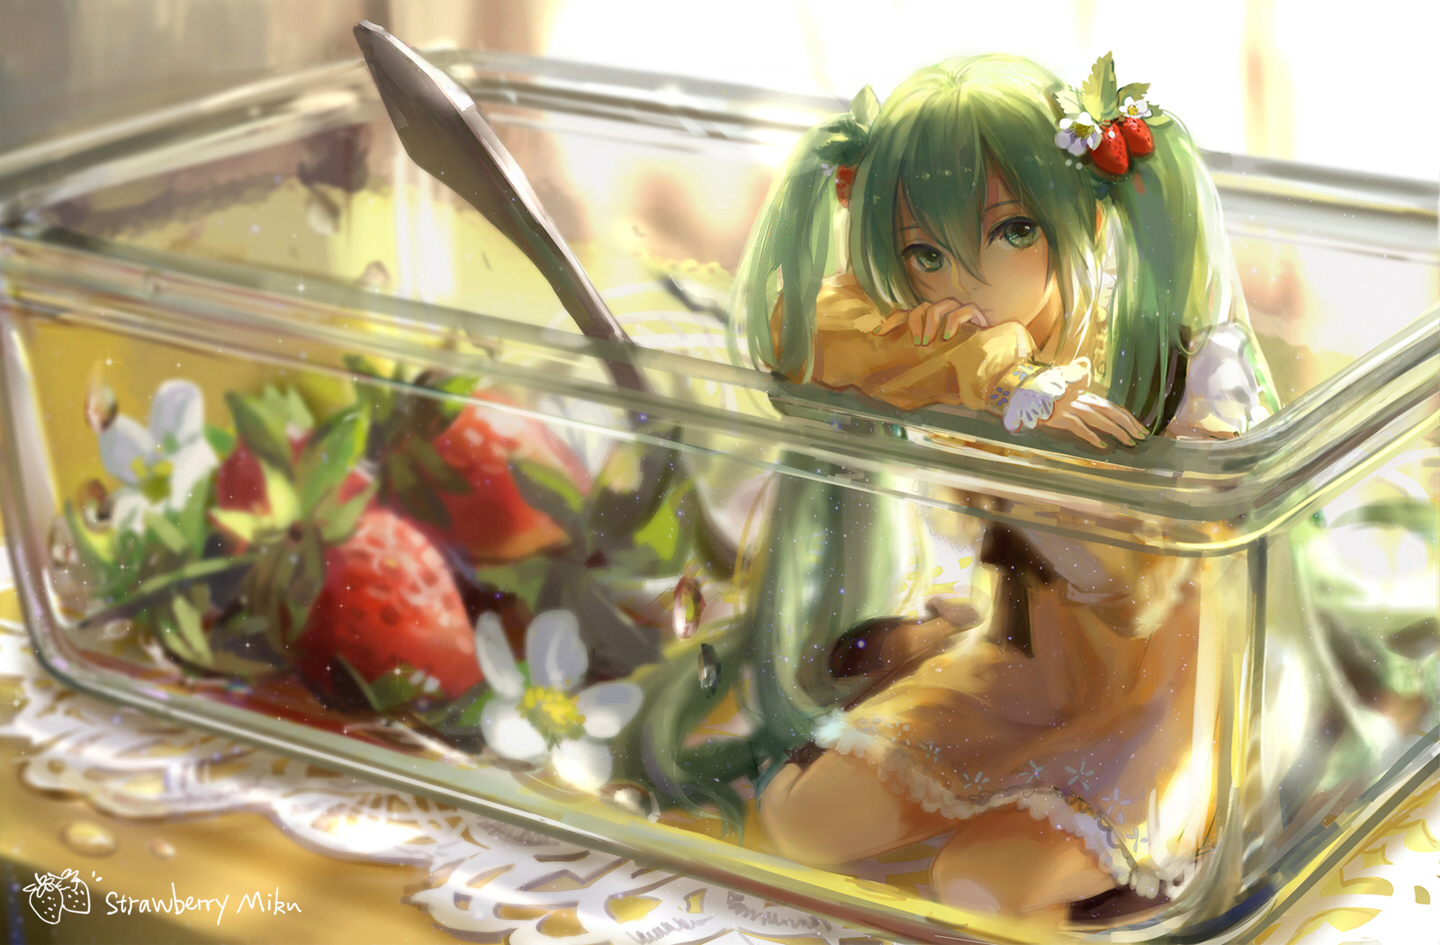
\includegraphics[scale=0.80]{43749408_p0.jpg}\end{center}
\note
\subsection{最长公共子序列---LCS}
\subsubsection{介绍与实现}
\begin{definition}[最长公共子序列]
一个数列,如果分别是两个或多个已知数列的子序列,且是所有符合此条件序列中最长的,则称为已知序列的最长公共子序列。在计算机科学中,最长递增子序列是指,在一个给定的数值序列中,找到一个子序列,使得这个子序列元素的数值依次递增,并且这个子序列的长度尽可能地大。
\end{definition}

以上是对最长公共子序列问题的定义。理解一下。

考虑一下这种题目如何打暴力。

非常容易,对吧,就是暴力枚举第一个序列的每一个子序列,对每一个子序列判断它是否为第二个序列的子序列。然而这样的时间复杂度是$O(2^{\min(n,m)})$的,其中n, m为字符串的长度。

思考这样一个性质:如果一个LCS是另一个LCS的前缀,那么一定存在一个LCS,使得它的长度为这两个LCS长度之和。

\begin{thm}[LCS的最优子结构]
	令$X=\langle x_1, x_2, \cdots, x_m\rangle$和$Y=\langle y_1, y_2,$ $\cdots,y_n\rangle$为两个序列,$Z=\langle z_1, z_2, \cdots, z_k\rangle$为X和Y的任意LCS。
	\begin{enumerate}
		\item{如果$x_m=y_n$,则$z_k=x_m=y_n$。且$Z_{k-1}$是$X_{m-1}$和$Y_{n-1}$的一个LCS。}
		\item{如果$x_m\neq y_n$,那么$x_m\neq y_n$意味着$Z$是$X_{m-1}$和$Y$的一个LCS。}
		\item{如果$x_m\neq y_n$,那么$z_k\neq y_n$意味着$Z$是$X$和$Y_{n-1}$的一个LCS。}
	\end{enumerate}
\end{thm}

举个例子:
\begin{center}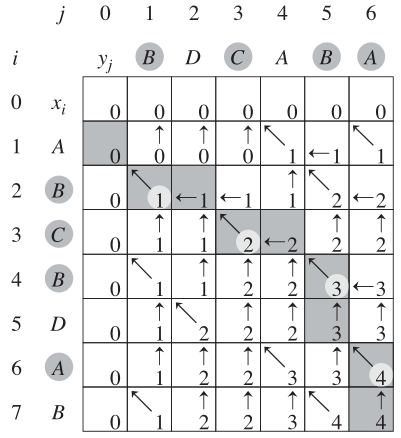
\includegraphics[height=5cm]{CLRS_LCS.png}\end{center}

上图是求$X=\langle A, B, C, D, B, D, A, B\rangle$和$B=\langle B, D, C, A, B, A\rangle$的LCS的过程。

\begin{Proof}
	(1)如果$z_k\neq x_m$,那么可以将$x_m=y_n$追加到$Z$的末尾,得到$X$和$Y$的一个长度为$k+1$的公共子序列。与$Z$是$X$和$Y$的最长公共子序列的假设矛盾。因此,必然有$z_k=x_m=y_n$。这样,前缀$Z_{k-1}$是$X_{m-1}$和$T_{n-1}$的一个长度为$k-1$的公共子序列。我们希望证明它是一个LCS。利用反证法,假设存在$X_{m-1}$和$Y_{n-1}$的一个长度大于$k-1$的公共子序列$W$,则将$x_m=y_n$追加到$W$的末尾会得到$X$和$Y$的一个长度大于$k$的公共子序列,矛盾。

	(2)如果$z_k\neq x_m$,那么$Z$是$X_{m-1}$和$Y$的一个公共子序列。如果存在$X_{m-1}$和Y的一个长度大于$k$的公共子序列$W$,那么$W$也是$X_m$和$Y$的公共子序列,与$Z$是$X$和$Y$的最长公共子序列的假设矛盾。

	(3)与情况(2)对称。\
\end{Proof}

于是我们get到了LCS的一个很重要的性质,没有后效性,具有最优子结构的性质。这是LCS问题可以DP的基础。

很容易看出,最初我们写的暴力求解算法中,有大量重叠的子问题(考虑求子序列$X = \langle x_a, x_{a+1}, \cdots, x_b\rangle$的LCS,必定求这个子序列的子序列$Y = \langle x_{a+m}, x_{a+m+1}, \cdots, x_{a+n}\rangle$这个子序列的LCS),所以LCS问题也有重叠子问题性质。

由上述定理我们就可以写出一个递归解。刚才的暴力中我们是枚举每一个子序列,然后进行判断,现在我们考虑能否直接构造出这样的一个序列。

明显的,状态转移有以下两种:
\begin{itemize}
	\item{如果两位相等,那么新的LCS可以连接到旧的LCS之后,构成一个新的较长的LCS。}
	\item{如果两位不相等,那么新的LCS不变,还是前一位的最长的LCS。}
\end{itemize}
设状态f[i][j]表示到字符串X的第i位与字符串Y的第j位的LCS长度,则:
\begin{equation*}
	f[i][j]=\begin{cases}
		f[i-1][j-1]+1             & , X[i]=Y[j]     \\
		\max(f[i][j-1],f[i-1][j]) & , X[i]\neq Y[j].
	\end{cases}
\end{equation*}

根据上面的状态转移方程写出代码即可,时间复杂度$O(nm)$.
\subsubsection{LCS的打印}
同LIS的打印,记录一下转移的方向,然后就可以了,时间复杂度为$O(nm)$。
\subsubsection{LCS的优化}
考虑一下是不是有什么地方还可以优化。

考虑上一节说的LCS的打印的过程,也可以不记录下转移的方向,因为每个状态转移的方向都是固定的,所以可以在$O(1)$的时间内判断出一个状态是由三个状态中的哪一个转移而来的,因此不再需要pre[]数组,只需要在输出过程中逆序转移,判断一下转移方向,把每一个数丢到栈里,再依次输出即可。

对于不需要输出LCS的问题,还可以使用滚动数组优化一下f数组的空间占用。因为每次转移只用到了f数组当前的一行以及前一行,所以只需要保留这两行数据即可。但是如果需要计算LCS的元素,就不能使用滚动数组优化(思考一下为什么)。

例题的话,可以参考一下洛谷P1439 的前50\%,至于后面的优化,建议参考一下题解,因为严格意义上这个优化意义不是很大,常数也很大,不是那么实用。
\begin{center}
\includegraphics[scale=0.08]{21804232_p0.jpg}\end{center}
\note
\section*{\textcolor{white}{?????}}
\begin{quote}
	\textcolor{white}{\ruby{千本}{せんぼん}\ruby{桜}{ざくら} \ruby{夜}{よる}ニ\ruby{紛}{まぎ}レ\\
		千本樱溶入夜中}

	\textcolor{white}{\ruby{君}{きみ}ノ\ruby{声}{こえ}モ\ruby{届}{とど}カナイヨ\\
		连你的声音也传不到啊}

	\textcolor{white}{\ruby{此処}{ここ}は\ruby{宴}{うたげ} \ruby{鋼}{はがね}の\ruby{檻}{おり}\\
		此处开宴钢铁牢笼中}

	\textcolor{white}{その\ruby{断頭台}{だんとうだい}で\ruby{見下}{みお}ろして\\
		自那断头台上往下看吧}

	\ \\

	\textcolor{white}{\ruby{三千}{さんぜん}\ruby{世界}{せかい} \ruby{常世}{とこよ}\ruby{之}{の}\ruby{闇}{やみ}\\
		三千世界黄泉之暗}

	\textcolor{white}{\ruby{嘆}{なげ}ク\ruby{唄}{うた}モ\ruby{聞}{き}コエナイヨ\\
		连哀叹之歌也听不见啊}

	\textcolor{white}{\ruby{青}{せい}\ruby{藍}{らん}の\ruby{空}{そら} \ruby{遥}{はる}か\ruby{彼方}かなた\\
		青蓝天空遥远彼端}

	\textcolor{white}{その\ruby{光線}{こうせん}\ruby{銃}{じゅう}で\ruby{打}{うち}\ruby{抜}{ぬ}いて\\
		就用那光线枪射穿吧}

	\begin{flushright}\textcolor{white}{------「千本桜」}\end{flushright}
\end{quote}
\newpage
\section{动态规划初步------背包问题}
这一部分,我们将开始对背包问题的研究。

准备好了吗?

限于篇幅以及我的姿势水平,在这一部分里我们仅研究最基础的动态规划问题。本人的目的不是想让你们通过这节课精通DP,而是想让你们对于DP有一个初步的了解,会做基本的DP题,并懂得举一反三,更重要的是\textbf{理解DP的思想}。
\subsection{背包问题是什么?}
\begin{definition}[背包问题(Knapsack problem)]是一种组合优化的NP完全问题。问题可以描述为:给定一组物品,每种物品都有自己的重量和价格,在限定的总重量内,我们如何选择,才能使得物品的总价格最高。
\end{definition}

以上就是百度百科对背包问题的定义,所谓“NP完全问题”是指这个问题具有多项式解法,即时间复杂度可以写成多项式形式$O(n^k\ , n \in\ $\textbf{N}$_+$
且$k$为已知常数$)$。背包问题本质上就是一种最优化组合问题,符合DP的要求,所以DP可以完成对背包问题的求解。时间复杂度是$O(n^2)$,空间复杂度是$O(n^2)$,优化后可以做到$O(n)$。

背包问题可以分为以下8类:
\begin{itemize}
	\item{01背包问题}
	\item{完全背包问题}
	\item{多重背包问题}
	\item{混合背包问题}
	\item{二维背包问题}
	\item{分组背包问题}
	\item{有依赖的背包问题}
	\item{泛化物品}
\end{itemize}

每种问题都有类似的做法,同时也有它们各自的不同之处。下面我们从最基础的01背包开始讲起,它非常重要,是后面所有背包问题的基础,一定要掌握。

\subsection{01背包问题}
\subsubsection{简介}
\begin{definition}[01背包问题]一个背包总容量为$V$,现在有$N$个物品,第$i$个物品体积为$weight[i]$,价值为$value[i]$,现在往背包里面装东西,怎么装能使背包的内物品价值最大?\end{definition}

以上就是\rm{01}背包的定义了。

看到此类问题,我们的第一反应大概就是贪心了。然而贪心是肯定不行的。

为什么不行?举一个例子:
\begin{example}最少硬币找零问题:给予不同面值的硬币若干种(每种硬币个数无限多),用若干种硬币组合为某种面额的钱,使硬币的的个数最少。\end{example}

在现实生活中,我们往往使用的是贪心算法,比如找零时需要13元,我们先找10元,再找2元,再找1元。这是因为现实生活中的硬币(纸币)种类特殊。如果我们的零钱可用的有1、2、5、9、10。我们找零18元时,贪心算法的策略是:10+5+2+1,四种,但是明明可以用两个9元的啊。所以肯定不能用贪心。

那么我们该怎么办?dalao们思考两分钟,不然我们先想一想搜索的方法吧(如果秒掉了的话就看看下面的图)。

\begin{center}
\includegraphics[scale=0.8]{6081163_p0.jpg}\end{center}
\newpage
\begin{example}\rm{01}背包问题:有$n$个重量和价值分别为$w[i]$和$v[i]$的物品。从这些物品中挑出总重量不超过$W$的物品,求所有挑选方案中价值总和的最大值。\end{example}

\subsubsection{搜索}
相信dalao们都能一眼秒掉这个问题。利用搜索,我们可以很快解决这个问题。代码如下:
\begin{enumerate}
\item \begin{minted}{C++}
void dfs(int index,int sumw,int sumv)//index:数组下标,sumw:当前情况的物品体积,sumv:当前情况的物品价值
{ 
    if(index>n)  
    {  
        if(sumw<=T&&sumv>maxvalue)  
            maxvalue=sumv;  
        return;  
    }  
    dfs(index+1,sumw+w[index],sumv+v[index]);//选
    dfs(index+1,sumw,sumv);//不选
}\end{minted}
\item \begin{minted}{C++}  
int W, n;
int w[MAXN], v[MAXN];  
int dfs(int i, int j)
{  
    int res;  
    if(i == n) res = 0;   
    else if(j < w[i]) res = dfs(i+1, j);  
    else res = max(dfs(i+1, j), dfs(i+1, j-w[i])+v[i]);  
    return res;  
}
\end{minted}
\end{enumerate}
然而以上代码有一个问题。时间复杂度太高,$O(2^n)$显然不能满足我们的要求,不能只过$n\leq15$的这部分数据啊。

考虑优化一下。记忆化搜索?
\begin{minted}{C++}
int W, n;    
int w[MAXN], v[MAXN];  
int dp[MAXN][MAXN];  
int dfs(int i, int j)
{  
    if(dp[i][j] >= 0) return dp[i][j];  
    int res;   
    if(i == n) res = 0; 
    else if(j < w[i]) res = dfs(i+1, j);   
    else res = max(dfs(i+1, j), dfs(i+1, j-w[i])+v[i]);  
    return dp[i][j] = res;  
}
\end{minted}

开一个二维数组记录一下每次搜索到的结果,这样时间复杂度就降低到了$O(nW)$,似乎不错。
\subsubsection{二维DP}
不然把上面的那个递归转化一下,转化成递推?简化一下代码?

设状态$dp[i+1][j]$表示从前$i$个物品挑选出总重量超过$j$的物品时,背包中的最大价值,那么根据题意,我们有以下递推式(就是状态转移方程):
\begin{equation*}
	dp[i+1][j]=\begin{cases}
		dp[i][j]                        & ,j<w[i]   \\
		\max\{dp[i+1][j],dp[j-w[i]]+v[i]\} & ,其他情况.
	\end{cases}
\end{equation*}

我来解释一下上面的状态转移方程。首先,要明确状态以及状态之间的转移过程。容易看到,在DFS中状态有两个参数$i,j$,分别代表\underline{当前是第几}\\\underline{个物品}以及\underline{当前背包的剩余容量}。所以DP也应该有两个状态,含义相同。如果背包容量不足了,那么就不取,价值不变;否则有两种决策:
\begin{itemize}
	\item{取当前物品,背包剩余容量减当前物品的体积,当前所获得价值加当前物品的价值;}
	\item{不取当前物品,考虑下一个物品。}
\end{itemize}

在这两种决策中取一个最优解即可。DP同理,只是将决策写成递推式的形式,本质和搜索是相同的。

所以我们得到以下代码:

\begin{minted}{C++}
for(int i = 0; i < N; ++i)
        for(int j = 0; j <= W; ++j)
            if(j < w[i])
                dp[i][j] = dp[i + 1][j];
            else
                dp[i][j] = max(dp[i + 1][j], dp[i + 1][j - w[i]] + v[i]);
\end{minted}
\textbf{重要提示:}\textcolor{red}{在DP中有一点非常重要,那就是\underline{\textbf{对状态数组的初始化}},万万不可忽略!在本题中,如果我们将数组开成全局变量,那么就不需要(\textbf{而不是可以忽略!})对状态数组的初始化,因为初始状态什么都没有放,价值都为0,同时全局变量默认的初始值都是0。\textbf{这只是一个个例!}很多题目都是\textbf{需要}对状态数组进行初始化的。在做DP题时,一定要先对初始状态进行初始化,否则\textbf{你极有可能获得0分,即使你的状态转移方程没有推错!}}
\subsubsection{一维DP}
考虑将前面的二维DP优化一下。

好像时间复杂度已经是最优化了,但是空间复杂度好像还有待提升。

看看刚才的状态转移方程或者代码。转移前后的状态有什么关系?

共同之处在于:$dp[i][j]=dp[i+1][Something]$,通过这个性质,我们可以压去这个方程的第一维,并且不取新的物品与背包没有空间时的情况相同,所以我们可以得到以下状态转移方程:
\begin{equation*}dp[i]=\max\{dp[i],dp[i-w[j]]+v[j]\},\ i\geq w[j]\end{equation*}

时间复杂度:$O(n^2)$,空间复杂度$O(n)$。

这个状态转移方程非常重要,在以后的学习中还会多次用到。

有什么问题随时问我就好,我会很乐意帮忙的。有不会的必须弄明白,因为01背包问题是所有其他背包问题的基础。

\textbf{重要提示:}\textcolor{red}{\textbf{请特别注意此题的枚举顺序,由于$dp[i]$是由$dp[i-w[j]]$转移来的,为了避免后效性需要倒序枚举背包的容量,这也是压维优化DP的特征}}(但不是所有的压维优化DP都需要倒序枚举)。

\note
\section*{\textcolor{white}{?????}}
\begin{quote}
	\textcolor{white}{やがて\ruby{日}{ひ}が\ruby{過}{す}ぎ \ruby{年}{とし}が\ruby{過}{す}ぎ\\
		光阴飞逝 岁月如梭}

	\textcolor{white}{\ruby{古}{ふる}い\ruby{荷物}{にもつ}も ふえて\\
		陈旧的负担 增加了}

	\textcolor{white}{あなたが かわっても\\
		你即使 自己改变}

	\textcolor{white}{\ruby{失}{な}くしたくないものは\\
		也不愿失去的事物}

	\textcolor{white}{ワタシに あずけてね\\
		就交由我 来保管吧}

	\ \\

	\textcolor{white}{\ruby{時}{とき}の\ruby{流}{なが}れも \ruby{傷}{きず}の\ruby{痛}{いた}みも\\
		不论是时间的流逝 受伤的苦痛}

	\textcolor{white}{\ruby{愛}{あい}の\ruby{深}{ふか}さも あなたの\ruby{声}{こえ}も\\
		爱意的深切 还是你的话声}

	\textcolor{white}{ワタシは\ruby{知}{し}らない だけど\ruby{歌}{うた}は\\
		即使我全都一无所知 依然继续地}

	\textcolor{white}{\ruby{歌}{うた}はうたえるわ だからきいて\\
		尽我所能的歌唱 所以请好好倾听吧}

	\textcolor{white}{もしもあなたが \ruby{望}{のぞ}むのなら\\
		若是你如此 期望的话}

	\textcolor{white}{\ruby{何}{なん}\ruby{度}{ど}でも \ruby{何}{なん}\ruby{度}{ど}だって\\
		不论几次 不论多少次}

	\textcolor{white}{かわらないわ あのときのまま\\
		不会改变的 从那时以来不曾变过的}

	\textcolor{white}{ハジメテノオトのまま...\\
		那不变的初次歌声...}

	\begin{flushright}\textcolor{white}{------「ハジメテノオト」}\end{flushright}
\end{quote}

\subsection{完全背包问题、多重背包问题与混合背包问题}
这一节内容看起来会比较多,但是因为有了前面一节的基础,相信大家也能够很容易的掌握。

\begin{definition}[完全背包问题]一个背包总容量为V,现在有N个物品,第i个物品体积为weight[i],价值为value[i],每个物品都有无限多件,现在往背包里面装东西,怎么装能使背包的内物品价值最大?\end{definition}

\begin{definition}[多重背包问题]一个背包总容量为V,现在有N个物品,第i个物品体积为weight[i],价值为value[i],每个物品有num[i]($num[i]\geq 1$)件,现在往背包里面装东西,怎么装能使背包的内物品价值最大?\end{definition}

\begin{definition}[混合背包问题]一个背包总容量为V,现在有N个物品,第i个物品体积为weight[i],价值为value[i],有的物品只有一件,有的物品有num[i]($num[i]\geq 1$)件,有的物品有无限多件,现在往背包里面装东西,怎么装能使背包的内物品价值最大?\end{definition}

以上是对这三种背包问题的定义,希望大家能够理解。可以发现这三种问题非常类似,也有不同。下面我就逐一来讲解。

\subsubsection{完全背包问题}

还记得上一节讲的01背包的一维状态转移方程吗?当时我曾经说过“为了避免后效性需要倒序枚举”,完全背包问题因为每个物品都有无限多件,所以可以利用这个后效性,正序枚举即可。

完全背包问题就讲完了。

\subsubsection{多重背包问题}
对于多重背包问题,我们可以考虑每一件物品都拆成01背包来做,N种物品,分别枚举每种物品的每一件即可。

就是加一层循环,枚举每一种物品中的每一件的状态。代码如下:
\begin{minted}{C++}
for(int i=0;i<N;i++)
    for(int j=0;j<num[i];j++)
        for(int k=V;k>=v[i];k--) 
            dp[k]=max(dp[k],dp[k-v[i]]+w[i]);
\end{minted}

这里稍微加了一点常数优化,注意最内层的循环,没有从V枚举到0,因为背包容量小于物品体积时对答案没有任何贡献(本来就放不下,当然不能硬塞)。

\subsubsection{混合背包问题}
这种问题就是把前面三种背包问题混合起来,所以我们只需要把前面三种背包都写一遍(实际上只要写完全背包和多重背包即可),然后加个判断就行了。

以下代码假设物品数量已经读入,第i个物品的数量用num[i]表示,且当num[i]=-1时,表示这个物品有无限多件:
\begin{minted}{C++}
for(int i=0;i<N;i++)
{
    if(num[i]!=-1)
    {
        for(int j=0;j<num[i];j++)
            for(int k=V;k>=v[i];k--) 
                dp[k]=max(dp[k],dp[k-v[i]]+w[i]);
	}
    else
    {
        for(int j=v[i];j<=V;j++)
            dp[j]=max(dp[j],dp[j-v[i]]+w[i]);
    }
}
\end{minted}

这三种问题是不是很简单呢?有不会的问题可以提问。
\note

\section*{\textcolor{white}{?????}}
\begin{quote}
	\textcolor{white}{\ruby{想}{おも}いよ\ruby{届}{とど}け \ruby{君}{きみ}に\\
		该怎么办才好…! 思念啊请传达给你}

	\ \par

	\textcolor{white}{お\ruby{願}{ねが}い\ruby{時間}{じかん}を\ruby{止}{とめ}めて \ruby{泣}{な}きそうなの\\
		拜托时间请停下来 感觉快要哭出来了}

	\textcolor{white}{でも\ruby{嬉}{うれ}しくて \ruby{死}{し}んでしまうわ!\\
		但是又好高兴 高兴到快要死掉了!}

	\ \par

	\textcolor{white}{メルト \ruby{駅}{えき}に\ruby{着}{つ}いてしまう……\\
		Melt 终究还是抵达了车站……}

	\ \par

	\textcolor{white}{もう\ruby{会}{あ}えない \ruby{近}{ちか}くて \ruby{遠}{とお}いよ だから\\
		再也见不到面了 那么的近 却又是那么的遥远 所以}

	\ \par

	\textcolor{white}{メルト \ruby{手}{て}をつないで\ruby{歩}{ある}きたい!\\
		Melt 想要手牵着手 一起前进!}

	\textcolor{white}{もうバイバイしなくちゃいけないの?\\
		已经是不得不说再见的时候了吗?}

	\ \par

	\textcolor{white}{\ruby{今}{いま}すぐ わたしを\ruby{抱}{だ}きしめて!\\
		现在马上 抱紧我!}

	\ \par

	\textcolor{white}{……なんてね\\
		……只是想想而已}
	\begin{flushright}\textcolor{white}{------メルト}\end{flushright}
\end{quote}
\newpage
\subsection{二维背包问题与分组背包问题}
\subsubsection{二维背包问题}
\begin{definition}[二维背包问题]对于每件物品,具有两种不同的费用;选择这件物品必须同时付出这两种代价;对于每种代价都有一个可付出的最大值(背包容量)。问怎样选择物品可以得到最大的价值。\end{definition}

定义比较长,但是事实上就是背包问题的再次综合。状态加一维表示第二种代价,然后套用适当的背包模板即可。注意最好使用一维的DP进行状态转移,否则可能会爆空间。


设第$i$件物品所需的两种代价分别为$a[i]$和$b[i]$。两种代价可付出的最大值(两种背包容量)分别为$u$和$v$。第$i$件物品的价值为$value[i]$。

三维状态转移方程:$f[i][u][v] = \max(f[i-1][u][v] , value[i] + f[i-1][u-a[i]][v-b[i]])$

二维状态转移方程(注意需要倒序枚举):$f[i][j] = \max(f[i][j] , value[k]$ $+ f[u-a[k]][v-b[k]])$

时间复杂度:$O(n^3)$,空间复杂度$O(n^2)$。

\subsubsection{分组背包问题}
\begin{definition}[分组背包问题]有N件物品和一个容量为V的背包。第i件物品的费用是w[i],价值是v[i]。这些物品被划分为k组,每组中的物品互相冲突,最多选一件。求解将哪些物品装入背包可使这些物品的费用总和不超过背包容量,且价值总和最大。\end{definition}

这种问题看起来与前面的问题不同。但实质是相同的。只不过枚举的对象由每一个物品变成每一类物品,然后对每一类物品分别枚举其中的每一个物品即可。

设枚举对象x为第1~k类物品,i为第x类物品中的第i件物品:

状态转移方程:$f[i]=\max\{f[i],f[i-w[i]]+v[i]\},i\in k_x.$
有问题随时问。
\note
\section*{\textcolor{white}{?????}}
\begin{quote}
	\textcolor{white}{\ruby{悲}{かな}しみの\ruby{海}{うみ}に\ruby{沈}{しず}んだ\ruby{私}{わたし} \ruby{目}{め}を\ruby{開}{あ}けるのも\ruby{億劫}{おっくう}\\
		沉入悲伤之海的我 就连想睁开眼也彷佛永劫}

	\textcolor{white}{このままどこまでも\ruby{堕}{お}ちて\ruby{行}{ゆ}き \ruby{誰}{だれ}にも\ruby{見}{み}つけられないのかな\\
		会就此沉沦下去 没人能够找到吗?}

	\ \par

	\textcolor{white}{どこへ\ruby{向}{む}かい、\ruby{何}{なに}をすれば? ふと\ruby{射}{さ}し\ruby{込}{こ}む\ruby{一筋}{ひとすじ}の\ruby{光}{ひかり}\\
		该朝向哪里,何去何从? 突然洒下的一丝光芒}

	\textcolor{white}{\ruby{手}{て}を\ruby{伸}{の}ばせば\ruby{届}{とど}きそうだけど \ruby{波}{なみ}に\ruby{拐}{さら}われて\ruby{見}{み}{失}{うしな}った\\
		虽然好像只要伸出手就能触及 却被海浪卷走失去踪影}

	\ \par

	\textcolor{white}{あれは\ruby{一体}{いったい}なんだったのかな あたたかくて\ruby{眩}{まぶ}しかったの\\
		那究竟是什么呢 既温暖又炫目}

	\textcolor{white}{\ruby{無}{む}{意}{い}{識}{しき}のカウンターイルミネーション\\
		无意识的对抗照明\\
		\ruby{嘘}{うそ}つきは\ruby{誰}{わだれ}?\\
		说谎的到底是谁?}

	\ \par

	\textcolor{white}{\ruby{深海}{しんかい}\ruby{少}{しょう}\ruby{女}{じょ} まだまだ\ruby{沈}{しず}む\\
		深海少女 仍在继续下沉}

	\textcolor{white}{\ruby{暗闇}{くらやみ}の{彼方}{かなた}へ\ruby{閉}{と}じこもる\\
	封闭在黑暗的彼端}

	\textcolor{white}{\ruby{深海}{しんかい}\ruby{少}{しょう}\ruby{女}{じょ} だけど\ruby{知}{し}りたい\\
		深海少女 但想要知道}

	\textcolor{white}{\ruby{心惹}{こころひ}かれるあの\ruby{人}{ひと}を\ruby{見}{み}つけたから\\
		只因找到了那令她倾心的人}
	\begin{flushright}\textcolor{white}{------深海少女}\end{flushright}
\end{quote}
\newpage
\subsection{有依赖的背包问题与泛化物品(选学)}
以下内容为选学,掌握与否都不很重要。讲解以经典例题为主\sout{,不能光\\讲基础的东西不讲题啊}。
\subsubsection{有依赖的背包问题}
\begin{example}金明的预算方案\\
	\textbf{题目描述}

	金明今天很开心,家里购置的新房就要领钥匙了,新房里有一间金明自己专用的很宽敞的房间。更让他高兴的是,妈妈昨天对他说:“你的房间需要购买哪些物品,怎么布置,你说了算,只要不超过N元钱就行”。今天一早,金明就开始做预算了,他把想买的物品分为两类:主件与附件,附件是从属于某个主件的,下表就是一些主件与附件的例子:
	\begin{center}
		\begin{tabular}{|c|c|}
			\hline
			主件   & 附件           \\
			\hline
			电脑   & 打印机、扫描仪 \\
			\hline
			书柜   & 图书           \\
			\hline
			书桌   & 台灯、文具     \\
			\hline
			工作椅 & 无             \\
			\hline
		\end{tabular}
	\end{center}

	如果要买归类为附件的物品,必须先买该附件所属的主件。每个主件可以有0个、1个或2个附件。附件不再有从属于自己的附件。金明想买的东西很多,肯定会超过妈妈限定的N元。于是,他把每件物品规定了一个重要度,分为5等:用整数1~5表示,第5等最重要。他还从因特网上查到了每件物品的价格(都是10元的整数倍)。他希望在不超过N元(可以等于N元)的前提下,使每件物品的价格与重要度的乘积的总和最大。

	设第j件物品的价格为v[j],重要度为w[j],共选中了k件物品,编号依次为$j_1,j_2,j_k$,则所求的总和为:
	\begin{equation*}
		v[j_1]\times w[j_1]+v[j_2]\times w[j_2]+ \cdots +v[j_k]\times w[j_k]
	\end{equation*}

	请你帮助金明设计一个满足要求的购物单。\\
	\textbf{输入输出格式}\\
	\textbf{输入格式}

	输入的第1行,为两个正整数,用一个空格隔开:

	N m (其中N($N<32000$)表示总钱数,m($m<60$)为希望购买物品的个数。)

	从第2行到第m+1行,第j行给出了编号为j-1的物品的基本数据,每行有3个非负整数

	v p q (其中v表示该物品的价格($v<10000$),p表示该物品的重要度(1~5),q表示该物品是主件还是附件。如果q=0,表示该物品为主件,如果q>0,表示该物品为附件,q是所属主件的编号)\\
	\textbf{输出格式}

	输出只有一个正整数,为不超过总钱数的物品的价格与重要度乘积的总和的最大值(不超过200000)。
	\par
	\ \\
	\textbf{输入输出样例}\\
	\textbf{输入样例}
	\begin{minted}{text}
1000 5
800 2 0
400 5 1
300 5 1
400 3 0
500 2 0
\end{minted}
	\textbf{输出样例}
	\begin{minted}{text}
2200
\end{minted}
\end{example}

这道例题是NOIp2006的提高组第二题。结合之前的讲解,dalao们有思路吗?先思考2分钟。

其实很简单,考虑状态:
\begin{itemize}
	\item{主件和两个附件都不选}
	\item{只选择主件,不选择任何一个附件}
	\item{选择主件并选择附件1}
	\item{选择主件并选择附件2}
	\item{选择主件和两个附件}
\end{itemize}

共计5个状态,所以大概需要写5个状态转移方程。

思路和正常向的01背包一致。

设每一件物品的属性:
\begin{itemize}
	\item{m:主件体积}
	\item{a:附件1体积}
	\item{b:附件2体积}
	\item{x:主件价值}
	\item{y:附件1价值}
	\item{z:附件2价值}
\end{itemize}
则我们可以得到:
\begin{eqnarray*}
	f[j]&=&\max(f[j],f[j-m[i]]+x[i])\\
	f[j]&=&\max(f[j],f[j-m[i]-a[i]]+x[i]+y[i])\\
	f[j]&=&\max(f[j],f[j-m[i]-b[i]]+x[i]+z[i])\\
	f[j]&=&\max(f[j],f[j-m[i]-a[i]-b[i]]+x[i]+y[i]+z[i])
\end{eqnarray*}

唯一需要注意的是边界条件(不能出现访问越界的错误)。

\subsubsection{泛化物品}
\begin{example}最佳课题选择\ \\
	\textbf{描述}

	Matrix67要在下个月交给老师n篇论文,论文的内容可以从m个课题中选择。由于课题数有限,Matrix67不得不重复选择一些课题。完成不同课题的论文所花的时间不同。具体地说,对于某个课题i,若Matrix67计划一共写x篇论文,则完成该课题的论文总共需要花费$A_i*x^{B_i}$个单位时间(系数$A_i$和指数$B_i$均为正整数)。给定与每一个课题相对应的$A_i$和$B_i$的值,请帮助Matrix67计算出如何选择论文的课题使得他可以花费最少的时间完成这n篇论文。\ \\
	\textbf{格式}\\
	\textbf{输入格式}

	第一行有两个用空格隔开的正整数n和m,分别代表需要完成的论文数和可供选择的课题数。

	以下m行每行有两个用空格隔开的正整数。其中,第i行的两个数分别代表与第i个课题相对应的时间系数Ai和指数Bi。\\
	\textbf{输出格式}

	输出完成n篇论文所需要耗费的最少时间。
	\ \\
	\textbf{样例}\\
	\textbf{样例输入}
	\begin{minted}{text}
10 3
2 1
1 2
2 1
\end{minted}
	\textbf{样例输出}
	\begin{minted}{text}
19
\end{minted}
	\textbf{数据范围}

	对于$30\%$的数据,$n\leq10, m\leq5$;

	对于$100\%$的数据,$n\leq200, m\leq20, A_i\leq100, B_i\leq5$。
\end{example}

这题非常经典,是泛化物品问题的一道好题。

首先给出泛化物品的定义:
\begin{definition}[泛化物品]在背包容量为V的背包问题中,泛化物品是一个定义域为$[0,V]$中的整数的函数h,当分配给它的费用为v时,能得到的价值就是h(v)。求能获得的最大价值。
\end{definition}

这题实际上不是很难,因为每件物品的数量都只能取整数,即函数$h(x)$的定义域为$x \in\ $\textbf{N}$_+$。所以我们只需要先预处理出$h(x)$在适当范围内的取值,然后套用适当的背包模板即可。

注意状态转移方程中加的部分是预处理出来的数组中对应的函数值。

\note
\section*{\textcolor{white}{?????}}
\begin{quote}
	\textcolor{white}{\ruby{何}{なに}も\ruby{伝}{つた}えないまま\\
		分毫的心意都没传达出}

	\textcolor{white}{さよならは\ruby{言}{い}えないよ\\
		这样子的我说不出再见}

	\ \par

	\textcolor{white}{この\ruby{声}{こえ} \ruby{枯}{か}れても\\
		即使这份 歌声凋零}

	\textcolor{white}{\ruby{消}{き}えない メロディー\\
		旋律依然 不会消失}

	\ \par

	\textcolor{white}{Last Night, Good Night\\
		Last Night, Good Night}

	\textcolor{white}{Last Night, Good Night\\
		Last Night, Good Night}

	\ \par

	\textcolor{white}{いつかは むかえる\\
		等待着那 随时可能}

	\textcolor{white}{\ruby{最後}{さいご}を \ruby{想}{おも}うよ\\
		会来临的 最后一刻}

	\textcolor{white}{\ruby{夜空}{よそら}に \ruby{願}{ねが}うの\\
		向着夜空 寄予心愿}

	\textcolor{white}{ときわの \ruby{笑顔}{えがお}を\\
		愿你永保 那份笑容}

	\textcolor{white}{おやすみ\\
		祝你好梦}
	\begin{flushright}\textcolor{white}{------}\em{\textcolor{white}{``Last Night, Good Night"}}\end{flushright}
\end{quote}

\newpage
\section{动态规划提高------棋盘型DP与区间型DP}
让我们再来看看稍微难一些的DP,这一部分先初步了解一下就行了,只要会了DP的思想,几乎所有的DP问题都能解决。

\subsection{棋盘型DP}
\begin{example} Likecloud-吃、吃、吃\\
	\textbf{题目背景}

	问世间,青春期为何物?

	答曰:“甲亢,甲亢,再甲亢;挨饿,挨饿,再挨饿!”\\
	\textbf{题目描述}

	正处在某一特定时期之中的李大水牛由于消化系统比较发达,最近一直处在饥饿的状态中。某日上课,正当他饿得头昏眼花之时,眼前突然闪现出了一个$n\times m$($n \and m\leq 200$)的矩型的巨型大餐桌,而自己正处在这个大餐桌的一侧的中点下边。餐桌被划分为了n*m个小方格,每一个方格中都有一个圆形的巨型大餐盘,上面盛满了令李大水牛朝思暮想的食物。李大水牛已将餐桌上所有的食物按其所能提供的能量打了分(有些是负的,因为吃了要拉肚子),他决定从自己所处的位置吃到餐桌的另一侧,但他吃东西有一个习惯——只吃自己前方或左前方或右前方的盘中的食物。

	由于李大水牛已饿得不想动脑了,而他又想获得最大的能量,因此,他将这个问题交给了你。

	每组数据的出发点都是最后一行的中间位置的下方!
	\ \\
	\textbf{输入输出格式}\\
	\textbf{输入格式:}

	第一行为m n.(n为奇数),李大水牛一开始在最后一行的中间的下方,接下来为$m\times n$的数字矩阵。

	共有m行,每行n个数字,数字间用空格隔开,代表该格子上的盘中的食物所能提供的能量。数字全是整数。\\
	\textbf{输出格式:}

	一个数,为你所找出的最大能量值。\\
	\textbf{输入输出样例}\\
	\textbf{输入样例}\ \\\ \\
	\begin{minted}{text}
6 7
16 4 3 12 6 0 3
4 -5 6 7 0 0 2
6 0 -1 -2 3 6 8
5 3 4 0 0 -2 7
-1 7 4 0 7 -5 6
0 -1 3 4 12 4 2
\end{minted}
	\textbf{输出样例}
	\begin{minted}{text}
41
\end{minted}
\end{example}

棋盘型DP大概就是给你一个棋盘,有一个人从某一个点出发,要求走到某一个点的什么东西。

针对这个题目,只需要设计出状态和方程就可以了。这个题目非常容易?设dp[i][j]表示当前吃到的格子能获得的最大能量,每一个格子都是由其左上方、正上方和右上方的格子转移而来。然后就可以轻易的得到状态转移方程:
\begin{equation*}f[i][j] = \max\{\max\{f[i-1][j-1],f[i-1][j]\},f[i-1][j+1]\} + map[i][j]\end{equation*}

这就完了。
\subsection{区间型DP}
\begin{example}{[USACO06FEB] Treats for the Cows 奶牛零食}\\
	\textbf{题目描述}

	FJ has purchased N (1 \leq N \leq 2000) yummy treats for the cows who get money for giving vast amounts of milk. FJ sells one treat per day and wants to maximize the money he receives over a given period time.

	The treats are interesting for many reasons:The treats are numbered 1..N and stored sequentially in single file in a long box that is open at both ends. On any day, FJ can retrieve one treat from either end of his stash of treats.Like fine wines and delicious cheeses, the treats improve with age and command greater prices.The treats are not uniform: some are better and have higher intrinsic value. Treat i has value v(i) (1 \leq v(i) \leq 1000).Cows pay more for treats that have aged longer: a cow will pay v(i)*a for a treat of age a.Given the values v(i) of each of the treats lined up in order of the index i in their box, what is the greatest value FJ can receive for them if he orders their sale optimally?

	The first treat is sold on day 1 and has age a=1. Each subsequent day increases the age by 1.

	约翰经常给产奶量高的奶牛发特殊津贴,于是很快奶牛们拥有了大笔不知该怎么花的钱.为此,约翰购置了N(1\leq N\leq 2000)份美味的零食来卖给奶牛们.每天约翰售出一份零食.当然约翰希望这些零食全部售出后能得到最大的收益.这些零食有以下这些有趣的特性:

	\begin{itemize}
		\item{零食按照$1\cdots N$编号,它们被排成一列放在一个很长的盒子里.盒子的两端都有开口,约翰每天可以从盒子的任一端取出最外面的一个。}
		\item{与美酒与好吃的奶酪相似,这些零食储存得越久就越好吃.当然,这样约翰就可以把它们卖出更高的价钱。}
		\item{每份零食的初始价值不一定相同.约翰进货时,第i份零食的初始价值为Vi($1\leq Vi\leq 1000$)。}
		\item{第i份零食如果在被买进后的第a天出售,则它的售价是$vi\times a$.}
	\end{itemize}
	Vi的是从盒子顶端往下的第i份零食的初始价值.约翰告诉了你所有零食的初始价值,并希望你能帮他计算一下,在这些零食全被卖出后,他最多能得到多少钱。\ \\
	\textbf{输入输出格式}\\
	\textbf{输入格式:}

	第1行:一个整数N。

	第2~N+1行:第i+1行包含零食i的价值vi。\\
	\textbf{输出格式:}

	一行一个数表示FJ在这些零食全被卖出后最多能得到的钱数。\\
	\textbf{输入输出样例}\\
	\textbf{输入样例:}

	\begin{minted}{text}
5
1
3
1
5
2
\end{minted}
	\textbf{输出样例:}
	\begin{minted}{text} 
43
\end{minted}
	\textbf{说明}

	样例解释:五个零食,在第一天FJ可以卖出1号零食(价值为1)或者5号零食(价值为2)。FJ按1,5,2,3,4顺序出售零食,获得的收益为$1\times 1+2\times 2+3\times 3+4\times 1+5\times 5=43$。
\end{example}

这题是个很经典的区间DP,区间DP的一般套路为设状态dp[l][r]为左端点为l,右端点为r区间[l,r]的值。

初始状态为:f[i][i]为自己第一天被取也就是v[i]*n,尝试往左右拓展即可。边界条件为取完所有元素(即序列为空的状态)。

状态转移方程:$f[l][r]=\max\{f[l][r-1]+v[r]*(n-i+1),f[l+1][r]+v[l]*(n-i+1)\}$.
\ \\ \par
于是这两种DP就都讲完了,相信大家对DP有了更深一步的了解。下面我们将学习更复杂的DP,可能是省选难度的DP了(不存在的,NOIp 2017就考了一道状压DP)。
\begin{center}
\includegraphics[scale=0.8]{47046948_p0.png}\end{center}
\note
\section{动态规划Professional------树形DP、状压DP与数位DP}
这一部分让我们看看\sout{非常水的}丧心病狂的DP类型,在NOIp 2017中首次出现了以前只出现在省选等高水平比赛中的DP类型------状压DP,这种类型的DP本质上是枚举状态(和搜索一样),但是又具有DP的某些特性。所以比较困难。树形DP则是另外一种不是很常见的DP类型,就是将DP的位置由矩阵上转移到树上来做。最后是最少见的数位DP。\sout{其实也不是非常难。}
\subsection{树形DP}
\begin{definition}[树形DP]就是把普通的DP转移到树上来做,转移方向就是由普通的在数组转移变为在树上借助边转移。其他的内容与普通DP无异。唯一需要注意的是\textcolor{red}{\textbf{先DP儿子节点}}。
\end{definition}

以上是对树形DP的定义,可以看出来它与普通的DP没什么区别。

为什么要先对儿子进行DP呢?其实非常简单,树的结构是由下而上越来越小的,如果先DP父亲节点,那么由于儿子节点还没有被更新,仍然保持初始值0,自然无法更新父亲节点。所以要先对较小规模的问题求解,即先处理依赖关系较少的节点(状态转移的基本性质,未知量由已知量转移而来)。

下面通过一道题目来说明一下树形DP的基本过程。
\begin{example}选课\\
	\textbf{题目描述}

	在大学里每个学生,为了达到一定的学分,必须从很多课程里选择一些课程来学习,在课程里有些课程必须在某些课程之前学习,如高等数学总是在其它课程之前学习。现在有N门功课,每门课有个学分,每门课有一门或没有直接先修课(若课程a是课程b的先修课即只有学完了课程a,才能学习课程b)。一个学生要从这些课程里选择M门课程学习,问他能获得的最大学分是多少?
	\ \\
	\textbf{输入输出格式}
	\ \\
	\textbf{输入格式:}

	第一行有两个整数N,M用空格隔开。(1<=N<=300,1<=M<=300)

	接下来的N行,第I+1行包含两个整数ki和si, ki表示第I门课的直接先修课,si表示第I门课的学分。若ki=0表示没有直接先修课(1<=ki<=N, 1<=si<=20)。
	\\
	\textbf{输出格式:}

	只有一行,选M门课程的最大得分。
	\\
	\textbf{输入输出样例}
	\\
	\textbf{输入样例:}
	\begin{minted}{text}
7  4
2  2
0  1
0  4
2  1
7  1
7  6
2  2
\end{minted}
	\textbf{输出样例:}
	\begin{minted}{text}
13
\end{minted}
\end{example}

题目大意是给定一个有依赖关系的课程安排表,一个课程可能依赖于多个课程,也可能被多个课程依赖,每学一个课程都能获得一些学分,最多学习M个课程,求能获得最大学分。

很明显,这是一个DAG(有向无环图),也就是一棵树。依赖关系可能不连续,也就是说给定的是一个森林。

对于森林的问题,我们可以通过虚拟一个总根节点,森林中所有的根节点都向这个总根节点连一条无向边,然后这个虚拟节点上的答案就是问题的答案。

因为树形数据结构是递归定义的(父亲节点与儿子节点,递归起点可以看做是根节点或某一个叶子节点,都可以遍历完整棵树),所以树形DP的基本思路应该是对树的每一个节点递推地计算该点的最优解,需要使用到DFS。

这道题的状态转移方程不难想到,设状态$f[i][j]$表示第i个节点取j个子节点(不包括自己)所取得的最大(最小)收益。然后标准状态转移模板就是$f[i][j]=\max(f[i][j],f[i][j-k]+f[儿子节点编号][k])$

现在考虑一下一棵子树的根节点可能会有多个儿子的情况。传统上有两种解决方案,第一种就是直接DFS,DP需要用到子树的时候就DFS这棵子树,不去考虑儿子的个数的问题。

这种做法的代码如下:
\begin{minted}{C++}
#include <cstdio>
#include <cstring>
#include <algorithm>
using namespace std;
int n,m,f[2005][2005];
int head[2005],next[2005],w[2005];
int dfs(int x){
    if (head[x]==-1) return 0;
    int sum=0;
    for (int i=head[x];i!=-1;i=next[i])
    {
        int t=dfs(i);
        sum+=t+1;
        for (int j=sum;j>=0;j--)
        {
            for (int k=0;k<=t;k++)
                if (j-k-1>=0) f[x][j]=max(f[x][j],f[x][j-k-1]+f[i][k]);
        }
    }
    return sum;
}
int main()
{
    scanf("%d%d",&n,&m);
    memset(f,0,sizeof(f));
    memset(head,-1,sizeof(head));
    for (int i=1;i<=n;i++)
    {
        int a;
        scanf("%d%d",&a,&w[i]);
        next[i]=head[a];
        head[a]=i;
    }
    for (int i=1;i<=n;i++) f[i][0]=w[i];
    f[0][0]=0;
    dfs(0);
    printf("%d",f[0][m]);
    return 0;
\end{minted}

另外一种做法是多叉树转为二叉树来做。多叉树转二叉树在树这一节内容lpy学姐已经给你们讲过了,就是左儿子右兄弟表示法,我就不讲了,直接说思路。

用f[root][k]表示第root节课为根且还剩k个自由选课数时,学分的最大值;
\begin{itemize}
	\item{不选此课,它与它的后续值皆为零;}
	\item{选此课,最终求max【它的值+兄弟与左孩子瓜分剩余选课数时最优解,原状态,不选它(但它兄弟的状态要与它合并,因为左孩子只有一个)】}
\end{itemize}

树形DP本质上是对这棵树的DFS操作。需要写个记忆化搜索优化一下。

于是就可以写出代码:

\begin{minted}{C++}
#include<cstdio>
#include<cstring>
using namespace std;
const int N=320;
int n,m;
int f[N][N],b[N],c[N],s[N];
void dp(int root,int k)
{
    if(f[root][k]>=0)return;
    if(root==0||k==0){f[root][k]=0;return;}
    dp(b[root],k);//兄弟与左孩子享有同等权利;
    for(int i=0;i<k;i++)
    {
        dp(c[root],k-i-1);//选第root门课; 
        dp(b[root],i);// 因为根节点给下一代指标时,只会给左孩子,所以下一代的左孩子要分给兄弟指标;
        f[root][k]=max(f[root][k], max(f[b[root]][k], f[b[root]][i] + f[c[root]][k - i - 1] + s[root]));
        //求三个状态最大值:选此状态(原封不动),不选,选此状态(更新,此节点+瓜分指标后的兄弟与左孩子的最优解) 
    }
}
int main()
{
    cin>>n>>m;
    int fa;
    for(int i=1;i<=n;i++)
    {
        cin>>fa>>s[i];
        if(fa==0)fa=n+1; 
        b[i]=c[fa];//c[i]记录的是长子,长子把‘长子’的位子让给i,原长子成为了新长子兄弟, 
        c[fa]=i;//父亲直辖原长子; 
    }
    memset(f,-1,sizeof(f));
    dp(c[n+1],m);
    cout<<f[c[n+1]][m];//无先修课的的最优值会集中于c[n+1]; 
    return 0;
}
\end{minted}
\begin{center}
\includegraphics[scale=1.75]{64304330_p0.png}\end{center}
\note
\subsection{状压DP}
\subsubsection{定义与特点}
\begin{definition}[状压DP]和普通的DP一样,同样需要设计状态与状态转移方程,保存一些状态来相互转移的解题过程,与普通DP不同的是,状压DP的状态不是简单的状态,而是\textbf{不同的方案}等等。状态压缩中的状态常用二进制来表示,转移过程常用位运算来完成。
\end{definition}

以上是我给状压DP的简单定义。或许不是非常准确,但是基本能反映出状压DP的含义了。如果不是特别理解的话,还是联想DP最初的定义,就是一个无限优化的搜索。只不过这个优化有点特殊,表示的状态与常见的DP有些不同。

状压DP的特点:\textcolor{red}{\textbf{数据范围非常小,一般有$n\leq 24$}},因为状压DP需要枚举每一个子集。

学习状压DP前首先需要了解位运算的相关知识。让我们先来看一下。
\subsubsection{有关位运算的知识}
设有一个集合$S$,用一个二进制数表示集合中每一个元素的选择情况(第$i$个二进制位为0表示不选集合$S$中的第$i$个元素,当然这个集合不具有数学上集合的无序性,要求是按编号有序排列的),则这个二进制数表示的是集合$S$的一个子集。

状压DP就是枚举子集,转移常常涉及对并集,交集、补集的操作。可以使用位运算来进行加速对集合的运算。

设有两个集合$S_1\subset S, S_2\subset S$,则我们有以下集合运算与位运算的关系:

\begin{center}
	\begin{tabular}{|c|c|}
		\hline
		集合运算               & 与之等价的位运算                   \\
		\hline
		$S_1\cap S_2$          & $S_1$ \verb+&+ $S_2$ \\
		\hline
		$S_1\cup S_2$          & $S_1$ \verb+|+ $S_2$ \\
		\hline
		$\complement_{S_1}S_2$ & $S_1$ \verb+^+ $S_2$ \\
		\hline
	\end{tabular}
\end{center}

状压的一些技巧:
\begin{itemize}
	\item{若S是U的子集,则S关于U的补集为:\verb$S^U$}
	\item{判断点$k$是否在集合S中(即S的第$k- 1$位是否为1):\\\verb$S&(1<<(k-1))!=0?"Yes":"No";$}
	\item{枚举S的子集:\verb$for(int i=S;i;i=(i-1)&S){...}$}
	\item{设置一个大小为n的全集:\verb$n=1<<(n-1)$}
\end{itemize}

下面给出两道例题,再细致地谈一下状压DP的内容和实现细节。

\subsubsection{基础例题---愤怒的小鸟}
\begin{example}愤怒的小鸟\\
\textbf{问题描述}

Kiana最近沉迷于一款神奇的游戏无法自拔。

简单来说,这款游戏是在一个平面上进行的。

有一架弹弓位于$(0,0)$处,每次Kiana可以用它向第一象限发射一只红色的小鸟,小鸟们的飞行轨迹均为形如$y=ax^2+bx$的曲线,其中a,b是Kiana指定的参数,且必须满足$a\leq 0$。

当小鸟落回地面(即x轴)时,它就会瞬间消失。

在游戏的某个关卡里,平面的第一象限中有n只绿色的小猪,其中第i只小猪所在的坐标为$(xi,yi)$。

如果某只小鸟的飞行轨迹经过了$(xi,yi)$,那么第i只小猪就会被消灭掉,同时小鸟将会沿着原先的轨迹继续飞行;

如果一只小鸟的飞行轨迹没有经过$(xi,yi)$,那么这只小鸟飞行的全过程就不会对第i只小猪产生任何影响。

例如,若两只小猪分别位于$(1,3)$和$(3,3)$,Kiana可以选择发射一只飞行轨迹为$y=-x^2+4x$的小鸟,这样两只小猪就会被这只小鸟一起消灭。

而这个游戏的目的,就是通过发射小鸟消灭所有的小猪。

这款神奇游戏的每个关卡对Kiana来说都很难,所以Kiana还输入了一些神秘的指令,使得自己能更轻松地完成这个游戏。这些指令将在【输入格式】中详述。

假设这款游戏一共有T个关卡,现在Kiana想知道,对于每一个关卡,至少需要发射多少只小鸟才能消灭所有的小猪。由于她不会算,所以希望由你告诉她。

\textbf【输入格式】

第一行包含一个正整数T,表示游戏的关卡总数。

下面依次输入这T个关卡的信息。每个关卡第一行包含两个非负整数n,m,分别表示该关卡中的小猪数量和Kiana输入的神秘指令类型。接下来的n行中,第i行包含两个正实数(xi,yi),表示第i只小猪坐标为(xi,yi)。数据保证同一个关卡中不存在两只坐标完全相同的小猪。

如果m=0,表示Kiana输入了一个没有任何作用的指令。

如果m=1,则这个关卡将会满足:至多用$\left \lceil \frac{n}{3} + 1 \right \rceil$只小鸟即可消灭所有小猪。

如果m=2,则这个关卡将会满足:一定存在一种最优解,其中有一只小鸟消灭了至少$\left \lfloor \frac{n}{3} \right \rfloor$只小猪。

保证$1\leq n\leq 18,0\leq m\leq 2,0\leq x_i,y_i\leq 10$,输入中的实数均保留到小数点后两位。

上文中,符号$\left \lceil x \right \rceil$和$\left \lfloor x \right \rfloor$分别表示对c向上取整和向下取整。\\
\textbf{【输出格式】}

对每个关卡依次输出一行答案。

输出的每一行包含一个正整数,表示相应的关卡中,消灭所有小猪最少需要的小鸟数量。\\
\textbf{【输入样例$1$】}
\begin{minted}{text}
2
2 0
1.00 3.00
3.00 3.00
5 2
1.00 5.00
2.00 8.00
3.00 9.00
4.00 8.00
5.00 5.00
\end{minted}
\textbf{【输出样例$1$】}
\begin{minted}{text}
1
1
\end{minted}
\textbf{【输入样例$2$】}
\begin{minted}{text}
3
2 0
1.41 2.00
1.73 3.00
3 0
1.11 1.41
2.34 1.79
2.98 1.49
5 0
2.72 2.72
2.72 3.14
3.14 2.72
3.14 3.14
5.00 5.00
\end{minted}
\textbf{【输出样例$2$】}
\begin{minted}{text}
2
2
3
\end{minted}
\textbf{【输入样例$3$】}
\begin{minted}{text}
1
10 0
7.16 6.28
2.02 0.38
8.33 7.78
7.68 2.09
7.46 7.86
5.77 7.44
8.24 6.72
4.42 5.11
5.42 7.79
8.15 4.99
\end{minted}
\textbf{输出样例$3$}
\begin{minted}{text}
6
\end{minted}
\textbf{【说明】}\\
\textbf{【样例解释1】}

这组数据中一共有两个关卡。

第一个关卡与【问题描述】中的情形相同,2只小猪分别位于$(1.00,3.00)$和$(3.00,3.00)$,只需发射一只飞行轨迹为$y = -x^2 + 4x$的小鸟即可消灭它们。

第二个关卡中有$5$只小猪,但经过观察我们可以发现它们的坐标都在抛物线 $y = -x^2 + 6x$上,故Kiana只需要发射一只小鸟即可消灭所有小猪。
\ \\
\textbf{【数据范围】}
\begin{center}
\begin{tabular}{c|c|c|c}
\Xhline{1.2pt}
测试点编号&$n$&$m$&$t$\\
\Xhline{1.2pt}
$1$&\multirow{2}{*}{$\leq 2$}&\multirow{12}{*}{$=0$}&$\leq 10$\\
\cline{1-1}\cline{4-4}
$2$&&&$\leq 30$\\
\cline{1-2}\cline{4-4}
$3$&\mr{2}{$\leq 3$}&&$\leq 30$\\
\cline{1-1}\cline{4-4}
$4$&&&$\leq 30$\\
\cline{1-2}\cline{4-4}
$5$&\mr{2}{$\leq 4$}&&$\leq 10$\\
\cline{1-1}\cline{4-4}
$6$&&&$\leq 30$\\
\cline{1-2}\cline{4-4}
$7$&$\leq 5$&&\mr{4}{$\leq 10$}\\
\cline{1-2}
$8$&$\leq 6$&&\\
\cline{1-2}
$9$&$\leq 7$&&\\
\cline{1-2}
$10$&$\leq 8$&&\\
\cline{1-2}\cline{4-4}
$11$&$\leq 9$&&\mr{4}{$\leq 30$}\\
\cline{1-2}
$12$&$\leq 10$&&\\
\cline{1-3}
$13$&\mr{2}{$\leq 12$}&$=1$&\\
\cline{1-1}\cline{3-3}
$14$&&$=2$&\\
\cline{1-4}
$15$&\mr{3}{$\leq 15$}&$=0$&\mr{3}{$\leq 15$}\\
\cline{1-1}\cline{3-3}
$16$&&$=1$&\\
\cline{1-1}\cline{3-3}
$17$&&$=2$&\\
\cline{1-4}
$18$&\mr{3}{$\leq 18$}&$=0$&\mr{3}{$\leq 5$}\\
\cline{1-1}\cline{3-3}
$19$&&$=1$&\\
\cline{1-1}\cline{3-3}
$20$&&$=2$&\\
\Xhline{1.2pt}
\end{tabular}
\end{center}
\end{example}

考虑一下,有思路吗?

其实这个数据范围,暴力也可以过。大家不妨先写个暴力玩玩。

因为状态的数目不是很多,所以我们考虑用二进制数来表示抛物线打掉的猪的集合。用0和1表示是否选中这一只猪,若二进制的第$i$位为表示选第$i$只猪,为1表示不选。举个例子,若使用32位有符号整数,即 \verb+int+ 类型表示一个状态,则二进制数 \verb+11111111111111111111111111111100B+ 表示的状态为打掉第一只猪和第二只猪所需抛物线的最少条数;而二进制数 \verb+111111111111111000000000000000000B+ 表示的状态为打掉第1到第18只猪所需抛物线的最少条数(注意有符号整数最高位是符号位,所以实际可用于表示集合的位数是31,如果开了 \verb+short+ 类型就对应题目中前17个数据)。

设状态$dp[S]$表示打掉集合$S$(用二进制表示)中所有的猪需要的最少小鸟数。状态的数目不是很多,可以考虑枚举每一条抛物线。一个贪心的思路是使每条抛物线都至少打掉两只猪,可以证明这样做是最优的(明显的,一次打两只猪要优于一次打只个猪)。枚举两只猪,如果它们不在同一列,代入这两只猪的坐标,解得$a$和$b$的值(可以使用加减消元法)。如果这组$a$和$b$没有出现过,那么就用这组$a$和$b$代入每一只猪看能否打到。于是我们就预处理出了$m$条抛物线能够打到的猪的编号的集合$S$,存入$a[]$数组。

我们的目标状态是打完所有的猪。也就是说答案是状态$dp[0]$的值。边界条件是$dp[2^n-1]=0$表示一头猪都不打的情况。然后由刚才预处理的$a[]$数组,我们可以得到状态转移方程:
\begin{equation*}
dp[i]=\min\!^m_{j=1}\{dp[i|a[j]],dp[i]\}+1, i|a[j]<dp[i].
\end{equation*}

\subsubsection{提高例题---宝藏}
\begin{example}宝藏\\
	\textbf{【问题描述】}

	参与考古挖掘的小明得到了一份藏宝图,藏宝图上标出了 n 个深埋在地下的宝藏屋,也给出了这 n 个宝藏屋之间可供开发的 m 条道路和它们的长度。

	小明决心亲自前往挖掘所有宝藏屋中的宝藏。但是,每个宝藏屋距离地面都很远, 也就是说,从地面打通一条到某个宝藏屋的道路是很困难的,而开发宝藏屋之间的道路则相对容易很多。

	小明的决心感动了考古挖掘的赞助商,赞助商决定免费赞助他打通一条从地面到某个宝藏屋的通道,通往哪个宝藏屋则由小明来决定。

	在此基础上,小明还需要考虑如何开凿宝藏屋之间的道路。已经开凿出的道路可以任意通行不消耗代价。每开凿出一条新道路,小明就会与考古队一起挖掘出由该条道路所能到达的宝藏屋的宝藏。另外,小明不想开发无用道路,即两个已经被挖掘过的宝藏屋之间的道路无需再开发。

	新开发一条道路的代价是:
	\begin{equation*}\mathrm{L} \times \mathrm{K}\end{equation*}

	L代表这条道路的长度,K代表从赞助商帮你打通的宝藏屋到这条道路起点的宝藏屋所经过的宝藏屋的数量(包括赞助商帮你打通的宝藏屋和这条道路起点的宝藏屋) 。

	请你编写程序为小明选定由赞助商打通的宝藏屋和之后开凿的道路,使得工程总代价最小,并输出这个最小值。
	\\
	\textbf{【输入格式】}

	第一行两个用空格分离的正整数 n 和 m,代表宝藏屋的个数和道路数。

	接下来 m 行,每行三个用空格分离的正整数,分别是由一条道路连接的两个宝藏屋的编号(编号为 1~n),和这条道路的长度 v。
	\ \\
	\textbf{【输出格式】}

	输出共一行,一个正整数,表示最小的总代价。
	\\
	\textbf{【输入输出样例】}
	\ \\
	\textbf{【输入样例$1$】}
	\begin{minted}{text}
4 5 
1 2 1 
1 3 3 
1 4 1 
2 3 4 
3 4 1 
\end{minted}
	\textbf{【输出样例$1$】}
	\begin{minted}{text}
4
\end{minted}
	\textbf{【输入样例$2$】}
	\begin{minted}{text}
4 5 
1 2 1 
1 3 3 
1 4 1 
2 3 4 
3 4 2  
\end{minted}
	\textbf{【输出样例$2$】}
	\begin{minted}{text}
5
\end{minted}
	\textbf{【说明】}
	\ \\
	\textbf{【样例解释$1$】}

	\begin{center}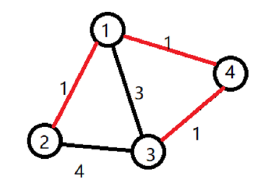
\includegraphics[width=5cm]{treasure_1.png}\end{center}
	小明选定让赞助商打通了 $1$ 号宝藏屋。小明开发了道路 $1 \to 2$,挖掘了 $2$ 号宝藏。开发了道路 $1 \to 4$,挖掘了 $4$ 号宝藏。还开发了道路 $4 \to 3$,挖掘了 $3$ 号宝藏。工程总代价为:$1 \times 1 + 1 \times 1 + 1 \times 2 = 4$
	\ \\
	\textbf{【样例解释$2$】}

	\begin{center}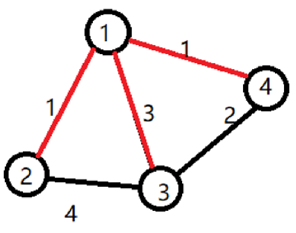
\includegraphics[width=5cm]{treasure_2.png}\end{center}

	小明选定让赞助商打通了 $1$ 号宝藏屋。小明开发了道路 $1 \to 2$,挖掘了 $2$ 号宝藏。开发了道路 $1 \to 3$,挖掘了 $3$ 号宝藏。还开发了道路 $1 \to 4$,挖掘了 $4$ 号宝藏。工程总代价为:$1 \times 1 + 3 \times 1 + 1 \times 1 = 5$
	\ \\
	\textbf{【数据规模与约定】}

	对于$20\%$的数据: 保证输入是一棵树,$1 \le n \le 8$,$v \le 5000$ 且所有的 v 都相等。

	对于$40\%$的数据: $1 \le n \le 8$,$0 \le m \le 1000$,$v \le 5000$ 且所有的 v 都相等。

	对于$70\%$的数据: $1 \le n \le 8$,$0 \le m \le 1000$,$v \le 5000$。

	对于$100\%$的数据: $1 \le n \le 12$,$0 \le m \le 1000$,$v \le 500000$。
\end{example}

一句话题意:
给定一个有重边,边有权值的无向图。从某一个点出发,求到达所有的点需要的最少费用,
并且限制两点之间只有一条路径。

费用的计算公式为:所有边的费用之和。而边(x\to y)的费用就为:y到初始点的距离 * 边权。

此题为NOIp 2017 Day2 T2。是一道比较基础的状压DP。有多种方法可以AC这道题目,正解有状压DP\sout{,模拟退火,遗传算法等等}。

会讲多种算法的。
\paragraph{随机化暴力}
dalao们应该都学习过搜索。搜索本质上就是个暴力。数据范围这么小,搜索是可以通过大部分数据的。是很划算的。

考虑随机一个点序列(在DFS时不按照输入顺序从1到n依次遍历整张图,容易被卡),然后指定一个定点为起点进行DFS计算出当前的花费(当然不一定要对整张图进行一次DFS,稍微剪一下枝),符合题意时更新一下答案就行了。当然这种算法在RP不好的时候会输出最大值,但这就是小概率事件了,况且可以多次对这个图进行随机化DFS。

考虑DFS的终止条件,由于我们希望图是一棵树(此时边数最小并且任意两点都可达),所以终止条件应该是找到了一棵树,即当前已经DFS过的点数等于$n+1$(联系最小生成树理解一下?)。

代码:
\begin{minted}{C++}
#include<cctype>
#include<cstdio>
#include<algorithm>
using namespace std;
#define N 20
#define fr(_a,_b,_c) for(int _a=_b;_a<=_c;_a++)
inline int read()
{
	char ch=getchar();int ret=0,flag=1;
	while(!isdigit(ch)&&ch!='-')ch=getchar();
	if(ch=='-')flag=-1;
	while(isdigit(ch))ret=ret*10+ch-'0',ch=getchar();
	return flag*ret;
}
int n,m,d[N][N],ans,t[N],h[N];
void dfs(int x,int w)//x表示当前DFS过的点的个数,w表示当前状态下的花费。
{
    if(ans<=w)//剪枝:如果已经找到的答案比当前状态下的花费小,回溯。
        return;
    if(x==n+1)//更新解,如果DFS到了一棵树并且需要更新答案,更新答案。
    {
        ans=w;
        return;
    }
    for(int i=1;i<=x-1;i++)
        if(d[t[x]][t[i]]+1)
        {
            h[t[x]]=h[t[i]]+1;
            dfs(x+1,w+d[t[x]][t[i]]*h[t[x]]);
        }
}
int main()
{
    n=read();
    m=read();
    fr(i,1,n)
        fr(j,1,n)
            d[i][j]=-1;
    fr(i,1,m)
    {
        int u=read(),v=read(),w=read();
        if(d[u][v]==-1)
            d[u][v]=d[v][u]=w;
        else
            d[u][v]=d[v][u]=min(d[u][v],w);
    }
    ans=(1<<20);
    fr(i,1,n)
        t[i]=i;
    srand((unsigned long long)new char);
    fr(i,1,5040)
    {
        fr(i,1,n*n)
            swap(t[rand()%n+1],t[rand()%n+1]);
        fr(i,1,n)
            h[i]=0;
        dfs(2,0);
    }
    printf("%d\n",ans);
    return 0;
}
\end{minted}

时间复杂度$O(5040\times 3^n)$,期望得分0~100.
\paragraph{模拟退火}
在介绍模拟退火算法之前先介绍一下TSP问题和TSP问题所属的NP问题和NPC问题。
\begin{definition}[NP问题] 是指存在多项式算法能够解决的非决定性问题,而其中NP完全问题又是最有可能不是P问题的问题类型。所有的NP问题都可以用多项式时间划归到他们中的一个。所以显然NP完全的问题具有如下性质:它可以在多项式时间内求解,当且仅当所有的其他的NP完全问题也可以在多项式时间内求解。
\end{definition}
以上是NP问题的定义,所谓多项式算法就是时间复杂度可以写作$O(n^a), $\\$a\in \mathbf{R}$的形式的算法。
\begin{definition}[NPC问题]NP中的某些问题的复杂性与整个类的复杂性相关联。这些问题中任何一个如果存在多项式时间的算法,那么所有NP问题都是多项式时间可解的。这些问题被称为NP完全问题(NPC问题)。
\end{definition}
	以上是对NPC问题的定义,换句话说就是不容易有有效算法的问题(需要搜索、枚举等等很暴力的算法来解决的问题)。
	\begin{definition}[TSP问题]又译为旅行推销员问题、货郎担问题,是数学领域中著名问题之一。问题的一般形式类似于“假设有一个旅行商人要拜访n个城市,他必须选择所要走的路径,路径的限制是每个城市只能拜访一次,而且最后要回到原来出发的城市。路径的选择目标是要求得的路径路程为所有路径之中的最小值。”

		\textbf{TSP问题可以被证明是一个NPC问题。}
	\end{definition}
	以上是对TSP问题的定义,要注意到这是一个NPC问题。
	\begin{definition}[模拟退火算法]是一种通用概率演算法,用来在一个大的搜寻空间内找寻命题的最优解。模拟退火算法是解决TSP(旅行商问题)的有效方法之一。

		模拟退火的出发点是基于物理中固体物质的退火过程与一般组合优化问题之间的相似性。模拟退火算法是一种通用的优化算法,其物理退火过程由加温过程、等温过程、冷却过程这三部分组成。
	\end{definition}
	可以看到,模拟退火是解决需要搜索的问题的一种有效算法(但是只针对于部分问题,不具有普适性)。

	转回来看这个题,由于答案具有比较强的连续性(可能与随机数据等等有关),所以模拟退火算法适用于这道题目。

	考虑下图所示的函数图像:
	\begin{center}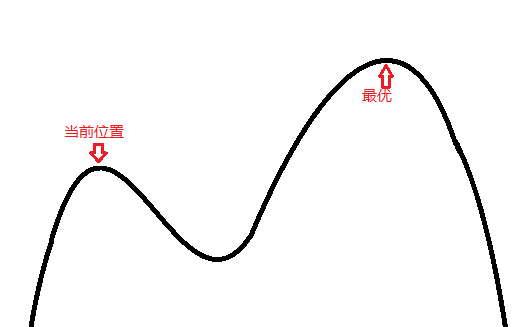
\includegraphics[scale=0.3]{sa.png}\end{center}
	如果坚决不接受较差的解,那么我们就无法到达最优解所在的位置。这使我们必须接受存在较差的解(但不能全部接受,否则就与搜索一样了)。我们可以写一个接受函数来决定是否接受这个解。假设答案越小越优,我们可以得到以下接受函数:
	\begin{minted}{C++}
bool accept(double delta, double temper)//delta表示函数的变化量,temper表示当前“温度”,“温度”随时间推移缓慢减小,从而实现“退火”的过程。
{
    if(delta <= 0) return true;//如果找到了更优的解,就接受。
    return rand() <= exp((-delta) / temper) * RAND_MAX;//随机接受较差的解。
}
\end{minted}
	下面解释一下第二行接受较差的解的代码:

	我们将$\textrm{rand()}\leq \exp(\frac{-\Delta}{temper})\times\textrm{RAND\_MAX}$移项,可得:
$\frac{\textrm{rand()}}{\textrm{RAND\_MAX}}\leq\exp(\frac{-\Delta}{temper})$,根据定义$temper$始终为正,而$\Delta$为正数,所以$\exp()$函数的自变量为负数。由指数函数的定义,返回值应该在区间(0,1)之间,定为接受的概率。而左边随机生成了一个实数,如果比概率小就接受,否则就不接受。

	简单来说,就是随机化接受较差的解,从而达到到达最优解的过程。由于“温度”随时间推移缓慢减小,所以跳往较差解的概率也下降。

	模拟退火的原理是,通过赋予搜索过程一种时变且最终趋于零的概率突跳性,从而可有效避免陷入局部极小并最终趋于全局最优的串行结构的优化算法。由于这个原理的限制,模拟退火算法能找到的最优解可能不是最优解,但是与最优解已经非常相近了。这个特性比较适合做较高水平的比赛中的提交答案题,可能能艹掉标程,获得更高的分数。但是对于传统型题目,就很有可能WA掉。

	结合这题的代码理解一下模拟退火的流程:
	\begin{minted}{C++}
#include<bits/stdc++.h>
using namespace std;
const int maxn=110;
const int maxm=2010;
int mp[maxn][maxn],n,m,i,j,k,x,y,z,ans,s;
int a[maxn],b[maxn],c[maxn],ha[maxn],oldf,newf,vis[maxn];
double T;//模拟退火中的温度
int read()
{
    int tot=0,fh=1;
    char c=getchar();
    while((c-'0'<0)||(c-'0'>9)){if(c=='-')fh=-1;c=getchar();}
    while((c-'0'>=0)&&(c-'0'<=9)){tot=tot*10+c-'0';c=getchar();}
    return tot*fh;
}
int dfs(int x,int dep)//遍历这张图,x表示当前点的编号,dep表示当前遍历过的点的个数
{
    if (dep>13) return 0;//如果已经不是一棵树了,不符合题中“小明不想开发无用道路,即两个已经被挖掘过的宝藏屋之间的道路无需再开发”这一条件,进行剪枝。
    if (x!=s){vis[x]=dfs(c[x],dep+1);return vis[x];}//若还未到达终点就继续进行DFS。
    else return 1;//若到达终点表示这是一组可行解。
}
int check()
{
    int i;
    memset(vis,0,sizeof(vis));
    for (i=1;i<=n;i++)//以每一个点为起点进行DFS
    {
        if (vis[i]==0) vis[i]=dfs(i,1);//vis[i]表示以i号点为起点是否存在可行解。
        if (vis[i]==0) return 0;//不存在可行解
    }
    return 1;
}
int dfs2(int x)//用于计算$\sum L_i\times K_i$新值的搜索,x表示当前点的编号。
{
    if ((s==x)||(vis[x]!=0)) return vis[x];//如果是起点或者已经被访问过了就返回x点的深度。
    int t1=dfs2(c[x])+1;//记录深度,即题目中的K
    vis[x]=t1;//记录当前点的深度
    newf=newf+t1*mp[c[x]][x];//更新$\sum L_i\times K_i$的值
    return t1;
}
void getnewf()//对dfs2()的封装,用于计算$\sum L_i\times K_i$的值
{
    int i;
    newf=0;
    memset(vis,0,sizeof(vis));
    for (i=1;i<=n;i++)//以每个点为起点进行DFS
    {
        if (vis[i]==0) dfs2(i);//如果没被访问过,即当前点对答案的贡献还没有计算进去,就计算一下从当前点可以增广到的点的距离。
    }
}
void bfs(int x)//寻找近似解
{
    int l=1,r=1,i; a[l]=x; oldf=0; b[x]=0;
    memset(ha,-1,sizeof(ha)); ha[x]=0;
    while (l<=r)
    {
        for (i=1;i<=n;i++)
        {
            if ((ha[i]==-1)&&(mp[a[l]][i]!=1e9))//如果没有被增广过并且l与i之间有边
            {
                ha[i]=ha[a[l]]+1;//记录一下深度
                r++; a[r]=i;//入队
                b[i]=a[l];//记录一下父亲节点
                oldf=oldf+mp[a[l]][i]*ha[i];//计算原有的f函数
            }
        }
        l++;//旧节点出队
    }
    ans=min(ans,oldf);//两者取一个较小值。
}
int main()
{
    n=read(); m=read();
    for (i=1;i<=n;i++)
    {
        for (j=1;j<=n;j++)
        {
            if (i==j) mp[i][j]=0;
            else mp[i][j]=1e9;
        }
    }
    for (i=1;i<=m;i++)
    {
        x=read(); y=read(); z=read();
        mp[x][y]=min(mp[x][y],z);
        mp[y][x]=min(mp[y][x],z);
    }
    ans=1e9;
    srand(19260817);
    for (i=1;i<=n;i++)
    {
        s=i; bfs(i);//以每个点为起点进行一次BFS计算深度。
        if (n<=2) continue;//如果只有两个点,就不需要退火。
        for (T=10000;T>=0.00001;T=T*0.9999)//模拟退火过程,T表示温度。
        {
            x=(rand()%(n-1))+1; if (x>=i) x++;//随机指定起点和终点。
            y=(rand()%(n-1))+1;
            if (y>=x) y++;
            if (mp[x][y]==1e9) continue;//不连通
            for (j=1;j<=n;j++) c[j]=b[j];//复制一下b数组
            c[x]=y;//起点的父亲节点是终点。
            if (check()==0) continue;//如果不存在可行解跳出循环
            getnewf();//计算新的代价
            if ((newf<=oldf)||( exp((oldf-newf)/T))>=((rand()%1000000)/1000000.0))//接受函数,解释见上。
            {
                ans=min(ans,newf);//更新一下答案
                for (j=1;j<=n;j++) b[j]=c[j];//复制一下c数组
                oldf=newf;//刚刚计算出的函数值变成旧的函数值
            }
        }
    }
    printf("%d\n",ans);
    return 0;
}
\end{minted}

	时间复杂度$O(207223n^3)$.
	\paragraph{最小生成树}
	这是考场上很多人想到的非完美解法,当时在考场上好像是可以过1号样例,但是2号样例过不了。我在考场上也想到了这种方法,然而并没有写完,所以gg。

	考虑一下最小生成树的问题所在。Kruskal算法需要贪心地选择边权较小的边,所以如果枚举的点不在最小生成树上,贪心的结果就是错误的。

	就是说,如果到某一个点的最优路径不在最小生成树上(因为不仅仅是最小生成树上的点,如果一条边在最小生成树上,但是他的深度非常深,那么它对答案的贡献,即L\times K就会非常大),答案就不对了。有一组数据可以卡掉Prim算法(当然据说Prim可以过大数据,yyf dalao写过Kruskal好像是没有分)。

	至于卡掉最小生成树的数据的话,rqy dalao出了一组:
	\begin{minted}{text}
7 7
1 2 5000
2 3 1
3 4 1
4 5 1
5 6 2
2 7 9
6 7 3 
\end{minted}
	\paragraph{状压DP}
	考虑一个事实,给定一个加点序列,上一节提出的贪心的策略就是正确的了(计算答案的过程转化成类似最短路的东西)。

	所以枚举一下1~12的全排列,get到加点的序列,然后贪心就行了。

	但是这样时间复杂度就是$O(n!2^n)$,只能过一部分数据(可以拿到80分)。

	考虑题目要求构造一棵生成树,使得所有边的费用之和最小。问题转换为树上问题。

	设所有的点构成全集$U$,定义状态$f_{i,j}$表示考虑到树的第$i$层,前$i$层已选的点的集合为$S$(使用二进制压缩状态)的最小代价。

	状态的转移可以枚举所有不在S中的集合(令集合$S'\subseteq(\complement_U S)$,枚举集合$S'$)作为树的第$i+1$层。

	状态转移:
	\begin{equation*}
		dp[i][S]\to dp[i+1][S|S']+(i+1)\times shortestPath[S'][S]
	\end{equation*}

	其中$shortestPath[S'][S]$表示从集合$S'$到集合$S$的最短距离(需要提前用Floyd算法预处理两点间的最短路,然后处理出来),如果理解不了就看一下上面对集合间最短距离的定义,就是枚举集合$S$与集合$S'$所有点对(a,b)所在集合$P=\{p(a,b)\mid a\in S, b\in S', S\cap S'=\emptyset\}$,点对$p(a,b)$的最短路长度之和,程序中使用$pval$数组保存了每个点对之间的最短路,然后再转化成集合之间的距离,存储到$sval$数组里面。

	DP的顺序:由DP方程,由大到小枚举层数,然后枚举集合就行了。

	边界条件:枚举根节点,则$dp[0][1\text{<\!<}(root-1)]=0$。

	代码:
	\begin{minted}{C++}
#include<cstdio>
#include<algorithm>
using namespace std;
typedef long long LL;
const int INF = 1e7;
const int N = 13;
int n, m, g[N][N], u, v, p, U;
LL dp[N][1<<N], ans = 1e14, sval[1<<N][1<<N], pval[N][1<<N];
void init(int root)//初始化DP数组,建树,将边界条件设置好 
{
    for(int i = 0; i <= n; i++)
        for(int j = 0; j <= U; j++)
            dp[i][j] = INF;
    dp[0][1<<(root-1)] = 0;
}
int main()
{
    scanf("%d%d", &n, &m);
    U = (1 << n) - 1;
    for(int i = 1; i <= n; i++)//初始化图、DP数组、最短路数组 
        for(int j = 1; j <= n; j++)
            if(i ^ j)
                g[i][j] = INF;
    for(int i = 1; i <= n; i++)
        for(int j = 0; j <= U; j++)
            pval[i][j] = INF;
    for(int i = 0; i <= U; i++)
        for(int j = 0; j <= U; j++)
            sval[i][j] = INF;
    while(m--)//邻接矩阵加边,注意有重边的情况取较小值。 
    {
        scanf("%d%d%d", &u, &v, &p);
        g[u][v] = min(g[u][v], p);
        g[v][u] = min(g[v][u], p);
    }
    for(int i = 1; i <= n; i++)//预处理所有满足条件的点对(a,b)之间的最短路,使用Floyd算法 
        for(int j = 0; j <= U; j++)
            for(int k = 1; k <= n; k++)
                if(j & (1 << (k - 1)))
                    pval[i][j] = min(pval[i][j], 1ll*g[i][k]);
    for(int i = 0; i <= U; i++)//预处理集合之间的距离 
    {
        int C = i ^ U;//求出$\complement_U S$
        for(int s = C; s; s = (s - 1) & C)
        {
            LL temp = 0;
            for(int j = 1; j <= n; j++)
                if(s & (1 << (j - 1)))
                    temp += pval[j][i];
            sval[s][i] = temp >= INF ? INF : temp;
        }
    }
    for(int root = 1; root <= n; root++)//枚举每一个根 
    {
        init(root);
        for(int i = 0; i < n; i++)//枚举每一个点 
            for(int S = 0; S <= U; S++)//枚举每一个集合 
                if(dp[i][S] != INF)
                {
                    int C = S ^ U;//求出$\complement_U S$ 
                    for(int s = C; s; s = (s - 1) & C)
                        dp[i+1][S|s] = min(dp[i+1][S|s], dp[i][S] + (i + 1) * sval[s][S]);//这里的'|'运算符是对集合做的运算,相当于求集合的并。 
                }
        for(int i = 0; i < n; i++)  ans = min(ans, dp[i][U]);
    }
    printf("%lld", ans);
    return 0;
}
\end{minted}

	时间复杂度$O(n^2\times 2^n)=84934656<10^8$,可以通过所有数据。

	这样的话,状压DP就讲完了。还是有些难理解的,我讲的可能不是很清楚,课下好好理解一下吧。

	(其实状压DP一般可以用启发式搜索或者是记忆化搜索水过去,就像前面讲的随机化暴力和模拟退火算法一样)
	\note
	\subsection{数位DP}
	\subsubsection{基础知识}
	\begin{definition}[数位DP]数位dp是一种计数用的dp,一般就是要统计一个区间$[le,ri]$内满足一些条件数的个数。
	\end{definition}
	以上是对于数位DP的定义。

	做关于数位的题目首先考虑一下枚举方式:
	\begin{enumerate}
		\item{\begin{minted}{C++}
for(int i=le;i<=ri;i++)  
    if(right(i)) ans++;
\end{minted}
		      无法记忆化搜索。gg。}
		\item{控制上界,按位从高到低枚举。
		      注意枚举时从高位开始,前导零也要枚举。
		      需要注意的是枚举是从``00001"这样开始枚举,一直枚举到小于右边界。}
	\end{enumerate}
	
	基本的动态模板:
	\begin{minted}{C++}
typedef long long ll;  
int a[20];  
ll dp[20][state];//不同题目状态不同  
ll dfs(int pos,/*state变量*/,bool lead/*前导零*/,bool limit/*数位上界变量*/)//不是每个题都要判断前导零  
{  
    //递归边界,既然是按位枚举,最低位是0,那么pos==-1说明这个数我枚举完了  
    if(pos==-1) return 1;/*这里一般返回1,表示你枚举的这个数是合法的,那么这里就需要你在枚举时必须每一位都要满足题目条件,也就是说当前枚举到pos位,一定要保证前面已经枚举的数位是合法的。不过具体题目不同或者写法不同的话不一定要返回1 */  
    //第二个就是记忆化(在此前可能不同题目还能有一些剪枝)  
    if(!limit && !lead && dp[pos][state]!=-1) return dp[pos][state];  
    /*常规写法都是在没有限制的条件记忆化,这里与下面记录状态是对应,具体为什么是有条件的记忆化后面会讲*/  
    int up=limit?a[pos]:9;//根据limit判断枚举的上界up;这个的例子前面用213讲过了  
    ll ans=0;  
    //开始计数  
    for(int i=0;i<=up;i++)//枚举,然后把不同情况的个数加到ans就可以了  
    {  
        if(...)
        else if(...)  
        ans+=dfs(pos-1,/*状态转移*/,lead && i==0,limit && i==a[pos]) //最后两个变量传参都是这样写的  
        /*这里还算比较灵活,不过做几个题就觉得这里也是套路了 
        大概就是说,我当前数位枚举的数是i,然后根据题目的约束条件分类讨论 
        去计算不同情况下的个数,还有要根据state变量来保证i的合法性,比如题目 
        要求数位上不能有62连续出现,那么就是state就是要保存前一位pre,然后分类, 
        前一位如果是6那么这意味就不能是2,这里一定要保存枚举的这个数是合法*/  
    }  
    //计算完,记录状态  
    if(!limit && !lead) dp[pos][state]=ans;  
    /*这里对应上面的记忆化,在一定条件下时记录,保证一致性,当然如果约束条件不需要考虑lead,这里就是lead就完全不用考虑了*/  
    return ans;  
}  
ll solve(ll x)  
{  
    int pos=0;  
    while(x)//把数位都分解出来  
    {  
        a[pos++]=x%10;//个人老是喜欢编号为[0,pos),看不惯的就按自己习惯来,反正注意数位边界就行  
        x/=10;  
    }  
    return dfs(pos-1/*从最高位开始枚举*/,/*一系列状态 */,true,true);//刚开始最高位都是有限制并且有前导零的,显然比最高位还要高的一位视为0嘛  
}  
int main()  
{  
    ll le,ri;  
    while(~scanf("%lld%lld",&le,&ri))  
    {  
        //初始化dp数组为-1,这里还有更加优美的优化,后面讲  
        printf("%lld\n",solve(ri)-solve(le-1));  
    }  
}  
\end{minted}

	为了做到无遗漏的枚举,代码中的limit变量就是用于判断枚举位置。
	最重要的问题在于“枚举上界”。如果不能理解的话,举个例子:
	枚举上界为219。
	假设已经枚举最高位为1,因为$0\le 2$,所以十位上怎么枚举也不会超过上界,limit应该为false,表示对这一位的枚举没有上界限制;
	假设枚举最高位为2,此时对十位的枚举就应该有限制,枚举上界为1;
	(对高位的枚举对低位有影响。)
	当然对位数小于ri的数来说,怎么枚举也没有问题,需要枚举上。
	想想判limit与不判limit记忆化搜索的不同。
	假设没判limit,那么假设我们第一次枚举了百位是0,显然后面的枚举limit=false,也就是数位上0到9的枚举,然后当我十位枚举了1,此时考虑dp[0][1],就是枚举到个位,前一位是1的个数,显然dp[0][1]=9;(个位只有是1的时候是不满足的),这个状态记录下来,继续dfs,一直到百位枚举了2,十位枚举了1,显然此时递归到了pos=0,pre=1的层,而dp[0][1]的状态已经有了即dp[pos][pre]!=-1;此时程序直接return dp[0][1]了,然而显然是错的,因为此时是有limit的个位只能枚举0,根本没有9个数,这就是状态冲突了。有lead的时候可能出现冲突,这只是两个最基本的不同的题目可能还要加限制,反正宗旨都是让dp状态唯一。
	有两点需要说明:
	\begin{enumerate}
		\item{limit为true的情况并不会非常多,逐个进行判断也不会特别浪费时间,所以需要记录一下,以解决子问题重叠的问题。}
		\item{DP状态可以改为dp[pos][status][limit],给limit也记忆化,记录不同的limit的个数,这种方法一般是对的。有些题目需要这样优化。}
	\end{enumerate}
	还涉及另一个问题。因为仅仅限制了枚举的上界,求出来的值不一定是原来题目要求的区间内的答案(实际上是区间[0,ri]的答案),所以要对答案进行一些处理。
	\begin{minted}{C++}
int main()  
{  
    long long le,ri;  
    while(~scanf("%lld%lld",&le,&ri))  
        printf("%lld\n",solve(ri)-solve(le-1));  
}  
\end{minted}

	上面的代码事实上就是对区间[0,ri]与[li,ri]取一个交集的过程,由高中数学的集合运算法则$A\cap B=A(A\subseteq B)$而来。

	DP的话,同记忆化搜索。状态一般是与前面已经枚举的数位有关,并且往往是对连续$k$位有要求,就保存前面$k-1$位的状态,然后当前枚举第$k$位,和前$k-1$位恰好拼凑出完整的状态。当然如果状态是数位的和,就直接保存数位的前缀和。
	\subsubsection{入门例题---不要62}
	我们来看一道入门难度的例题。
	\begin{example}
		HDU2089 不要62\\
		\textbf{题目描述}

		杭州人称那些傻乎乎粘嗒嗒的人为62(音:laoer)。

		杭州交通管理局经常会扩充一些的士车牌照,新近出来一个好消息,以后上牌照,不再含有不吉利的数字了,这样一来,就可以消除个别的士司机和乘客的心理障碍,更安全地服务大众。

		不吉利的数字为所有含有4或62的号码。例如:\verb+62315 73418 88914+都属于不吉利号码。但是,61152虽然含有6和2,但不是62连号,所以不属于不吉利数字之列。

		你的任务是,对于每次给出的一个牌照区间号,推断出交管局今次又要实际上给多少辆新的士车上牌照了。\\
		\textbf{输入格式}

		输入的都是整数对n、m($0\leq n\leq m\leq 1000000$),如果遇到都是0的整数对,则输入结束。\\
		\textbf{输出格式}

		对于每个整数对,输出一个不含有不吉利数字的统计个数,该数值占一行位置。\\
		\textbf{样例输入}
		\begin{minted}{text}
1 100
0 0
\end{minted}
		\textbf{样例输出}
		\begin{minted}{text}
80
\end{minted}
	\end{example}

	就是数位上不能有4也不能有连续的62,没有4的话在枚举的时候判断一下,不枚举4就可以保证状态合法了,所以这个约束没有记忆化的必要,而对于62的话,涉及到两位,当前一位是6或者不是6这两种不同情况我计数是不相同的,所以要用状态来记录不同的方案数。

	dp[pos][sta]表示当前第pos位,前一位是否是6的状态,这里sta只需要去0和1两种状态就可以了,不是6的情况可视为同种,不会影响计数。
	
	代码:
	\begin{minted}{C++}
#include<iostream>  
#include<cstdio>  
#include<cstring>  
#include<string>  
using namespace std;  
typedef long long ll;  
int a[20];  
int dp[20][2];  
int dfs(int pos,int pre,int sta,bool limit)  
{  
    if(pos==-1) return 1;  
    if(!limit && dp[pos][sta]!=-1) return dp[pos][sta];  
    int up=limit ? a[pos] : 9;  
    int tmp=0;  
    for(int i=0;i<=up;i++)  
    {  
        if(pre==6 && i==2)continue;  
        if(i==4) continue;//都是保证枚举合法性  
        tmp+=dfs(pos-1,i,i==6,limit && i==a[pos]);  
    }  
    if(!limit) dp[pos][sta]=tmp;  
    return tmp;  
}  
int solve(int x)  
{  
    int pos=0;  
    while(x)  
    {  
        a[pos++]=x%10;  
        x/=10;  
    }  
    return dfs(pos-1,-1,0,true);  
}  
int main()  
{  
    int le,ri;  
    //memset(dp,-1,sizeof dp);可优化  
    while(~scanf("%d%d",&le,&ri) && le+ri)  
    {  
        memset(dp,-1,sizeof dp);  
        printf("%d\n",solve(ri)-solve(le-1));  
    }  
    return 0;  
}  
\end{minted}

	\sout{其实还是记忆化搜索。}
	\subsubsection{常数优化}
	讲一个常数优化,放在ACM赛制中比较好用。

	把memset放在多组数据以外。由于数位DP的特点,DP状态与数本身有关,而不是与数据的组数有关,所以之前的状态还可以继续使用。

	求数位和是10的倍数的个数,这里简化为数位sum\%10这个状态,即dp[pos][sum]这里10是与多组无关的,所以可以memset优化,不过注意如果题目的模数是输入的话那就不能这样了。
	\subsubsection{减法的艺术---F(x)}
	先来看一道例题。
	\begin{example} HDU4734 F(x)\\
	\textbf{题目描述}
	
	对于一个有$n$位的十进制数$x(A_nA_{n-1}A_{n-2}\cdots A_2A_1)$,我们定义它的权值为:
	\begin{equation*}
	F(x)=A_n\times 2^{n-1}+A_{n-1}\times 2^{n-1}+A_{n-2}\times 2^{n-2}+\cdots+A_2\times 2+A_1\times 1.
	\end{equation*}
	
给定两个数A和B,请计算在区间$[0,B]$内有多少个数权值不超过F(A)。\\
	\textbf{输入格式}
	
	第一行包含一个数$T(T\leq 10000)$,表示测试数据组数;
	
	对于每一组测试数据,都有两个数$A$和$B(0\leq A, B\leq 10^9)$。\\
	\textbf{输出格式}
	
	对于每一组数据,你应该先输出`` \verb+Case #t: + ''(不包含引号),$t$是测试数据编号,从$1$开始。然后输出答案。\\
	\textbf{样例输入}
\begin{minted}{text}
3
0 100
1 10
5 100
\end{minted}
\textbf{样例输出}
\begin{minted}{text}
Case #1: 1
Case #2: 2
Case #3: 13
\end{minted}
	\end{example}

常规想:这个f(x)计算就和数位计算是一样的,就是加了权值,所以dp[pos][sum],这状态是基本的。a是题目给定的,f(a)是变化的不过f(a)最大好像是4600的样子。如果要memset优化就要加一维存f(a)的不同取值,那就是dp[10][4600][4600],这显然不合法。

这个时候就要用减法了,dp[pos][sum],sum不是存当前枚举的数的前缀和(加权的),而是枚举到当前pos位,后面还需要凑sum的权值和的个数,也就是说初始的是时候sum是f(a),枚举一位就减去这一位在计算f(i)的权值,那么最后枚举完所有位 sum\leq 0时就是满足的,后面的位数凑足sum位就可以了。

仔细想想这个状态是与f(a)无关的,一个状态只有在sum\leq 0时才满足,如果我们按常规的思想求f(i)的话,那么最后sum\leq f(a)才是满足的条件。

这道题目展示了前缀和在数位DP中的重要作用。希望大家理解一下。以下是代码:
\begin{minted}{C++}
#include<cstdio>  
#include<cstring>  
#include<iostream>  
#include<string>  
  
using namespace std;  
const int N=1e4+5;  
int dp[12][N];  
int f(int x)  
{  
    if(x==0) return 0;  
    int ans=f(x/10);  
    return ans*2+(x%10);  
}  
int all;  
int a[12];  
int dfs(int pos,int sum,bool limit)  
{  
    if(pos==-1) {return sum<=all;}  
    if(sum>all) return 0;  
    if(!limit && dp[pos][all-sum]!=-1) return dp[pos][all-sum];  
    int up=limit ? a[pos] : 9;  
    int ans=0;  
    for(int i=0;i<=up;i++)  
    {  
        ans+=dfs(pos-1,sum+i*(1<<pos),limit && i==a[pos]);  
    }  
    if(!limit) dp[pos][all-sum]=ans;  
    return ans;  
}  
int solve(int x)  
{  
    int pos=0;  
    while(x)  
    {  
        a[pos++]=x%10;  
        x/=10;  
    }  
    return dfs(pos-1,0,true);  
}  
int main()  
{  
    int a,ri;  
    int T;  
    int kase=1;  
    scanf("%d",&T);  
    memset(dp,-1,sizeof dp);  
    while(T--)  
    {  
        scanf("%d%d",&a,&ri);  
        all=f(a);  
        printf("Case #%d: %d\n",kase++,solve(ri));  
    }  
    return 0;  
}  
\end{minted}
	\note
	\section{典型题目与难题选讲}
	\subsection{典型题目}
	这里给出几道基础的DP题目,大家尽情AK吧!
	\begin{itemize}
		\item{\href{https://www.luogu.org/problem/show?pid=1216}{[USACO1.5]数字三角形 Number Triangles}---例题}
		\item{\href{https://www.luogu.org/problem/show?pid=1508}{Likecloud-吃、吃、吃}---数字三角形}
		\item{\href{https://www.luogu.org/problem/show?pid=1064}{金明的预算方案}---例题}
		\item{\href{https://www.luogu.org/problem/show?pid=1002}{过河卒}---模拟式DP}
		\item{\href{https://www.luogu.org/problem/show?pid=1115}{最大子段和}--- DP或者贪心}
		\item{\href{https://www.luogu.org/problem/show?pid=1091}{合唱队形}---最长上升子序列+最长下降子序列}
		\item{\href{https://www.luogu.org/problem/show?pid=2782}{友好城市}---最长上升子序列}
		\item{\href{https://www.luogu.org/problem/show?pid=1020}{导弹拦截}---最长不下降子序列}
		\item{\href{https://www.luogu.org/problem/show?pid=1108}{低价购买}---最长下降子序列+统计}
		\item{\href{https://www.luogu.org/problem/show?pid=2285}{[HNOI2004]打鼹鼠}---最长上升子序列}
		\item{\href{https://www.luogu.org/problem/show?pid=2871}{[USACO07DEC]手链Charm Bracelet}---01背包模板题}
		\item{\href{https://www.luogu.org/problem/show?pid=1048}{采药}---01背包模板题}
		\item{\href{https://www.luogu.org/problem/show?pid=1060}{开心的金明}---01背包}
		\item{\href{https://www.luogu.org/problem/show?pid=2639}{[USACO09OCT]Bessie的体重问题Bessie's We...}---01背包}
		\item{\href{https://www.luogu.org/problem/show?pid=1926}{小书童——刷题大军}---01背包}
		\item{\href{https://www.luogu.org/problem/show?pid=1049}{装箱问题}---01背包}
		\item{\href{https://www.luogu.org/problem/show?pid=1616}{疯狂的采药}---完全背包}
		\item{\href{https://www.luogu.org/problem/show?pid=1757}{通天之分组背包}---分组背包}
		\item{\href{https://www.luogu.org/problem/show?pid=1507}{NASA的食物计划}---二维背包}
		\item{\href{https://www.luogu.org/problem/show?pid=1164}{小A点菜}---背包问题的变体}
		\item{\href{https://www.luogu.org/problem/show?pid=1156}{垃圾陷阱}---类背包DP}
		\item{\href{https://www.luogu.org/problem/show?pid=1280}{尼克的任务}---考虑枚举方向}
		\item{\href{https://www.luogu.org/problem/show?pid=1103}{书本整理}---转化}
		\item{\href{https://www.luogu.org/problem/show?pid=1725}{琪露诺}---DP的优化}
		\item{\href{https://www.luogu.org/problem/show?pid=2822}{组合数问题}---杨辉三角+前缀和}
	\end{itemize}

	题目有些多,但是还是最好一一刷完。最后4道题以及每个类型的最后一道题稍微有些难度。

	想要提升能力的话,可以尝试一下下面这些题目:
	\begin{itemize}
		\item{\href{https://www.luogu.org/problem/show?pid=1004}{方格取数}---双线程DP}
		\item{\href{https://www.luogu.org/problem/show?pid=1006}{传纸条}---双线程DP}
		\item{\href{https://www.luogu.org/problem/show?pid=1541}{乌龟棋}---较高维度的DP}
		\item{\href{https://www.luogu.org/problem/show?pid=1373}{小a和uim之大逃离}---较复杂的DP}
	\end{itemize}

	以上差不多有30道题的样子了。希望大家能抽时间做一下。

	\begin{center}
\includegraphics[scale=0.25]{33237093_p0.jpg}\end{center}

	\newpage
	\subsection{难题选讲}
	\subsubsection{组合数问题---数论/数学,DP,前缀和优化}
	\begin{example} 组合数问题\\
		\textbf{【问题描述】}

		组合数$C_n^m$表示的是从n个物品中选出m个物品的方案数。举个例子,从$\rm (1,2,3)$三个物品中选择两个物品可以有$\rm (1,2),(1,3),(2,3)$这三种选择方法。根据组合数的定义,我们可以给出计算组合数的一般公式:

		\begin{equation*}C_n^m=\frac{n!}{m!(n - m)!}\end{equation*}

		其中$n!=1\times 2\times\cdots\times n$。

		小葱想知道如果给定n,m和k,对于所有的$0\leq i\leq n$,$0\leq j\leq\min(i,m)$有多少对$\rm (i,j)$满足$C_i^j$是k的倍数。\\
		\textbf{【输入输出格式】}\\
		\textbf{【输入格式】}

		从文件 problem.in 中读入数据。

		第一行有两个整数$t,k$,其中$t$代表该测试点总共有多少组测试数据,$k$的意义见 【问题描述】。

		接下来$t$行每行两个整数$n, m$,其中$n, m$的意义见【问题描述】。 \\
		\textbf{【输出格式】}

		输出到文件problem.out中。

		t行,每行一个整数代表答案。\\
		\textbf{【输入输出样例】}\\
		\textbf{【输入样例1】}
		\begin{minted}{text}
1 2
3 3
\end{minted}
		\textbf{【输出样例1】}
		\begin{minted}{text}
1
\end{minted}
		\textbf{【输入样例2】}
		\begin{minted}{text}
2 5
4 5
6 7
\end{minted}
		\textbf{【输出样例2】}
		\begin{minted}{text}
0
7
\end{minted}
		\textbf{【说明】}\\
		\textbf{【样例$1$说明】}

		在所有可能的情况中,只有$C_2^1 = 2$是$2$的倍数。\\
		\textbf{【子任务】}

		子任务会给出部分测试数据的特点。如果你在解决题目中遇到了困难,可以尝试只解决一部分测试数据。

		每个测试点的数据规模及特点如下表:
		\begin{center}
			\begin{tabular}{c|c|c|c|c}
				\Xhline{1.2pt}
				测试点 & $n$                          & $m$                          & $k$   & $t$         \\
				\Xhline{1.2pt}
				$1$    & \multirow{2}{*}{$\leq 3$}    & \multirow{2}{*}{$\leq 3$}    & $=2$  & $=1$        \\
				\cline{1-1}\cline{4-5}
				$2$    &                              &                              & $=3$  & $\leq 10^4$ \\
				\hline
				$3$    & \multirow{2}{*}{$\leq 7$}    & \multirow{2}{*}{$\leq 7$}    & $=4$  & $=1$        \\
				\cline{1-1}\cline{4-5}
				$4$    &                              &                              & $=5$  & $\leq 10^4$ \\
				\hline
				$5$    & \multirow{2}{*}{$\leq 10$}   & \multirow{2}{*}{$\leq 10$}   & $=6$  & $=1$        \\
				\cline{1-1}\cline{4-5}
				$6$    &                              &                              & $=7$  & $\leq 10^4$ \\
				\hline
				$7$    & \multirow{2}{*}{$\leq 20$}   & \multirow{2}{*}{$\leq 100$}  & $=8$  & $=1$        \\
				\cline{1-1}\cline{4-5}
				$8$    &                              &                              & $=9$  & $\leq 10^4$ \\
				\hline
				$9$    & \multirow{2}{*}{$\leq 25$}   & \multirow{2}{*}{$\leq 2000$} & $=10$ & $=1$        \\
				\cline{1-1}\cline{4-5}
				$10$   &                              &                              & $=11$ & $\leq 10^4$ \\
				\hline
				$11$   & \multirow{2}{*}{$\leq 60$}   & \multirow{2}{*}{$\leq 20$}   & $=12$ & $=1$        \\
				\cline{1-1}\cline{4-5}
				$12$   &                              &                              & $=13$ & $\leq 10^4$ \\
				\hline
				$13$   & \multirow{4}{*}{$\leq 100$}  & \multirow{2}{*}{$\leq 25$}   & $=14$ & $=1$        \\
				\cline{1-1}\cline{4-5}
				$14$   &                              &                              & $=15$ & $\leq 10^4$ \\
				\cline{1-1}\cline{3-3}\cline{4-5}
				$15$   &                              & \multirow{2}{*}{$\leq 60$}   & $=16$ & $=1$        \\
				\cline{1-1}\cline{4-5}
				$16$   &                              &                              & $=17$ & $\leq 10^4$ \\
				\hline
				$17$   & \multirow{4}{*}{$\leq 2000$} & \multirow{2}{*}{$\leq 100$}  & $=18$ & $=1$        \\
				\cline{1-1}\cline{4-5}
				$18$   &                              &                              & $=19$ & $\leq 10^4$ \\
				\cline{1-1}\cline{3-3}\cline{4-5}
				$19$   &                              & \multirow{2}{*}{$\leq 2000$} & $=20$ & $=1$        \\
				\cline{1-1}\cline{4-5}
				$20$   &                              &                              & $=21$ & $\leq 10^4$ \\
				\Xhline{1.2pt}
			\end{tabular}
		\end{center}
	\end{example}

	这是一道数论题,暴力分也很多(50分)。

	我们可以先打个表(毕竟数论上来先打表),看看前若干项的值。

	手推一下样例二:
	\begin{equation*}
		\begin{matrix}
			C^0_0                                         \\
			C^0_1 & C^1_1                                 \\
			C^0_2 & C^1_2 & C^2_2                         \\
			C^0_3 & C^1_3 & C^2_3 & C^3_3                 \\
			C^0_4 & C^1_4 & C^2_4 & C^3_4 & C^4_4         \\
			C^0_5 & C^1_5 & C^2_5 & C^3_5 & C^4_5 & C^5_5
		\end{matrix}
	\end{equation*}

	套套公式,看看在数组中的存储(不符合组合数的定义处设为$-1$):
	\begin{equation*}
		\begin{matrix}
			-1 & 0 & 0  & 0  & 0  & 0 & 0 \\
			-1 & 1 & 0  & 0  & 0  & 0 & 0 \\
			-1 & 2 & 1  & 0  & 0  & 0 & 0 \\
			-1 & 3 & 3  & 1  & 0  & 0 & 0 \\
			-1 & 4 & 6  & 4  & 1  & 0 & 0 \\
			-1 & 5 & 10 & 10 & 5  & 1 & 0 \\
			-1 & 6 & 15 & 20 & 15 & 6 & 1
		\end{matrix}
	\end{equation*}

	容易看出这是一个杨辉三角。

	建立状态转移方程。$O(n^2)$求出杨辉三角。然后数组存储杨辉三角的对应项对k取模后的值即可。

	再开个数组,统计一下数组中有多少个0就行了。

	然后写一个前缀和优化一下,问题解决。

	时间复杂度$O(n^2)$。

	\note

	\subsubsection{换教室---期望DP}
	期望DP是最近几年新加入NOIp考纲的内容,于NOIp 2016试水,以后几年可能会比较常考。在这里只介绍最基础的一道题,来源是NOIp 2016 Day1 T3.

	\begin{example} 换教室\\
		\textbf{题目描述}

		对于刚上大学的牛牛来说,他面临的第一个问题是如何根据实际情况申请合适的课程。

		在可以选择的课程中,有 $2n$ 节课程安排在 $n$ 个时间段上。在第 $i$($1 \leq i \leq n$)个时间段上,两节内容相同的课程同时在不同的地点进行,其中,牛牛预先被安排在教室 $c_i$ 上课,而另一节课程在教室 $d_i$ 进行。

		在不提交任何申请的情况下,学生们需要按时间段的顺序依次完成所有的 $n$ 节安排好的课程。如果学生想更换第 $i$ 节课程的教室,则需要提出申请。若申请通过,学生就可以在第 $i$ 个时间段去教室 $d_i$ 上课,否则仍然在教室 $c_i$ 上课。

		由于更换教室的需求太多,申请不一定能获得通过。通过计算,牛牛发现申请更换第 $i$ 节课程的教室时,申请被通过的概率是一个已知的实数 $k_i$,并且对于不同课程的申请,被通过的概率是互相独立的。

		学校规定,所有的申请只能在学期开始前一次性提交,并且每个人只能选择至多 $m$ 节课程进行申请。这意味着牛牛必须一次性决定是否申请更换每节课的教室,而不能根据某些课程的申请结果来决定其他课程是否申请;牛牛可以申请自己最希望更换教室的 $m$ 门课程,也可以不用完这 $m$ 个申请的机会,甚至可以一门课程都不申请。

		因为不同的课程可能会被安排在不同的教室进行,所以牛牛需要利用课间时间从一间教室赶到另一间教室。

		牛牛所在的大学有 $v$ 个教室,有 $e$ 条道路。每条道路连接两间教室,并且是可以双向通行的。由于道路的长度和拥堵程度不同,通过不同的道路耗费的体力可能会有所不同。 当第 $i$($1 \leq i \leq n-1$)节课结束后,牛牛就会从这节课的教室出发,选择一条耗费体力最少的路径前往下一节课的教室。

		现在牛牛想知道,申请哪几门课程可以使他因在教室间移动耗费的体力值的总和的期望值最小,请你帮他求出这个最小值。\\
		\textbf{输入输出格式}\\
		\textbf{输入格式}

		第一行四个整数 $n,m,v,e$。$n$ 表示这个学期内的时间段的数量;$m$ 表示牛牛最多可以申请更换多少节课程的教室;$v$ 表示牛牛学校里教室的数量;$e$表示牛牛的学校里道路的数量。

		第二行 $n$ 个正整数,第 $i$($1 \leq i \leq n$)个正整数表示 $c_i$,即第 $i$ 个时间段牛牛被安排上课的教室;保证 $1 \le c_i \le v$。

		第三行 $n$ 个正整数,第 $i$($1 \leq i \leq n$)个正整数表示 $d_i$,即第 $i$ 个时间段另一间上同样课程的教室;保证 $1 \le d_i \le v$。

		第四行 $n$ 个实数,第 $i$($1 \leq i \leq n$)个实数表示 $k_i$,即牛牛申请在第 $i$ 个时间段更换教室获得通过的概率。保证 $0 \le k_i \le 1$。

		接下来 $e$ 行,每行三个正整数 $a_j, b_j, w_j$,表示有一条双向道路连接教室 $a_j, b_j$,通过这条道路需要耗费的体力值是 $w_j$;保证 $1 \le a_j, b_j \le v$, $1 \le w_j \le 100$。

		保证 $1 \leq n \leq 2000$,$0 \leq m \leq 2000$,$1 \leq v \leq 300$,$0 \leq e \leq 90000$。

		保证通过学校里的道路,从任何一间教室出发,都能到达其他所有的教室。

		保证输入的实数最多包含 $3$ 位小数。\\
		\textbf{输出格式}

		输出一行,包含一个实数,四舍五入精确到小数点后恰好$2$位,表示答案。你的输出必须和标准输出完全一样才算正确。

		测试数据保证四舍五入后的答案和准确答案的差的绝对值不大于 $4 \times 10^{-3}$。(如果你不知道什么是浮点误差,这段话可以理解为:对于大多数的算法,你可以正常地使用浮点数类型而不用对它进行特殊的处理)\ \\
		\textbf{输入输出样例}\\
		\textbf{输入样例}
		\begin{minted}{text}
3 2 3 3
2 1 2
1 2 1
0.8 0.2 0.5 
1 2 5
1 3 3
2 3 1
\end{minted}
		\textbf{输出样例}
		\begin{minted}{text}
2.80
\end{minted}
		\textbf{说明}\\
		【样例说明】

		所有可行的申请方案和期望收益如下表:
		\begin{center}
			\begin{tabular}{c|c|c|c}
				\Xhline{1.2pt}
				申请通过的时间段 & 出现的概率 & 耗费的体力值 & 耗费的体力值的期望      \\
				\Xhline{1.2pt}
				无               & $1.0$      & $8$          & $8.0$                   \\
				\hline
				$1$              & $0.8$      & $4$          & \multirow{2}{*}{$4.8$}  \\
				\cline{1-3}
				无               & $0.2$      & $8$          &                         \\
				\hline
				$2$              & $0.2$      & $0$          & \multirow{2}{*}{$6.4$}  \\
				\cline{1-3}
				无               & $0.8$      & $8$          &                         \\
				\hline
				$3$              & $0.5$      & $4$          & \multirow{2}{*}{$6.0$}  \\
				\cline{1-3}
				无               & $0.5$      & $8$          &                         \\
				\hline
				$1、2$           & $0.16$     & $4$          & \multirow{4}{*}{$4.48$} \\
				\cline{1-3}
				$1$              & $0.64$     & $4$          &                         \\
				\cline{1-3}
				$2$              & $0.04$     & $0$          &                         \\
				\cline{1-3}
				无               & $0.16$     & $8$          &                         \\
				\hline
				$1、3$           & $0.4$      & $0$          & \multirow{4}{*}{$2.8$}  \\
				\cline{1-3}
				$1$              & $0.4$      & $4$          &                         \\
				\cline{1-3}
				$3$              & $0.1$      & $4$          &                         \\
				\cline{1-3}
				无               & $0.1$      & $8$          &                         \\
				\hline
				$2、3$           & $0.1$      & $4$          & \multirow{4}{*}{$5.2$}  \\
				\cline{1-3}
				$2$              & $0.1$      & $0$          &                         \\
				\cline{1-3}
				$3$              & $0.4$      & $4$          &                         \\
				\cline{1-3}
				无               & $0.4$      & $8$          &                         \\
				\Xhline{1.2pt}
			\end{tabular}
		\end{center}
		【提示】

		$1.$道路中可能会有多条双向道路连接相同的两间教室。 也有可能有道路两端连接
		的是同一间教室。

		$2.$请注意区分n,m,v,e的意义, n不是教室的数量, m不是道路的数量。

		特殊性质$1$:图上任意两点 $a_i$, $b_i$, $a_i\neq b_i$间,存在一条耗费体力最少的路径只包含一条道路。

		特殊性质$2$:对于所有的 $1\leq i\leq n$, $k_i=1$ 。\\
		【子任务】

		\begin{center}
			\begin{tabular}{c|c|c|c|c|c}
				\Xhline{1.2pt}
				测试点 & $n$                          & $m$                          & $v$                         & 特殊性质1                & 特殊性质2                \\
				\Xhline{1.2pt}
				$1$    & $\leq 1$                     & $\leq 1$                     & $\leq 300$                  & \multirow{4}{*}{\times}  & \multirow{4}{*}{\times}  \\
				\cline{1-4}
				$2$    & \multirow{3}{*}{$\leq 2$}    & $\leq 0$                     & $\leq 20$                   &                          &                          \\
				\cline{1-1}
				$3$    &                              & $\leq 1$                     & $\leq 100$                  &                          &                          \\
				\cline{1-1}\cline{3-4}
				$4$    &                              & $\leq 2$                     & $\leq 300$                  &                          &                          \\
				\hline
				$5$    & \multirow{3}{*}{$\leq 3$}    & $\leq 0$                     & $\leq 20$                   & \multirow{2}{*}{$\surd$} & $\surd$                  \\
				\cline{1-1}\cline{3-4}\cline{6-6}
				$6$    &                              & $\leq 1$                     & $\leq 100$                  &                          & \multirow{2}{*}{\times}  \\
				\cline{1-1}\cline{3-5}
				$7$    &                              & $\leq 2$                     & \multirow{2}{*}{$\leq 300$} & \times                   &                          \\
				\cline{1-3}\cline{5-6}
				$8$    & \multirow{4}{*}{$\leq 10$}   & $\leq 0$                     &                             & \multirow{2}{*}{$\surd$} & $\surd$                  \\
				\cline{1-1}\cline{3-4}\cline{6-6}
				$9$    &                              & $\leq 1$                     & $\leq 20$                   &                          & \multirow{2}{*}{\times}  \\
				\cline{1-1}\cline{3-5}
				$10$   &                              & $\leq 2$                     & $\leq 100$                  & \multirow{2}{*}{\times}  &                          \\
				\cline{1-1}\cline{3-4}\cline{6-6}
				$11$   &                              & $\leq 10$                    & $\leq 300$                  &                          & $\surd$                  \\
				\hline
				$12$   & \multirow{4}{*}{$\leq 20$}   & $\leq 0$                     & $\leq 20$                   & $\surd$                  & \multirow{3}{*}{\times}  \\
				\cline{1-1}\cline{3-5}
				$13$   &                              & $\leq 1$                     & $\leq 100$                  & \times                   &                          \\
				\cline{1-1}\cline{3-5}
				$14$   &                              & $\leq 2$                     & \multirow{2}{*}{$\leq 300$} & $\surd$                                             \\
				\cline{1-1}\cline{3-3}\cline{5-6}
				$15$   &                              & $\leq 20$                    &                             & \multirow{3}{*}{\times}  & $\surd$                  \\
				\cline{1-4}\cline{6-6}
				$16$   & \multirow{4}{*}{$\leq 300$}  & $\leq 0$                     & $\leq 20$                   &                          & \multirow{2}{*}{\times}  \\
				\cline{1-1}\cline{3-4}
				$17$   &                              & $\leq 1$                     & $\leq 100$                  &                                                     \\
				\cline{1-1}\cline{3-6}
				$18$   &                              & $\leq 2$                     & \multirow{2}{*}{$\leq 300$} & $\surd$                  & \multirow{2}{*}{$\surd$} \\
				\cline{1-1}\cline{3-3}\cline{5-5}
				$19$   &                              & $\leq 300$                   &                             & \multirow{7}{*}{\times}  &                          \\
				\cline{1-4}\cline{6-6}
				$20$   & \multirow{6}{*}{$\leq 2000$} & $\leq 0$                     & \multirow{2}{*}{$\leq 20$}  &                          & \multirow{6}{*}{\times}  \\
				\cline{1-1}\cline{3-3}
				$21$   &                              & $\leq 1$                     &                             &                          &                          \\
				\cline{1-1}\cline{3-4}
				$22$   &                              & $\leq 2$                     & \multirow{2}{*}{$\leq 100$} &                                                     \\
				\cline{1-1}\cline{3-3}
				$23$   &                              & \multirow{3}{*}{$\leq 2000$} &                             &                          &                          \\
				\cline{1-1}\cline{4-4}
				$24$   &                              &                              & \multirow{2}{*}{$\leq 300$} &                                                     \\
				\cline{1-1}
				$25$   &                              &                              &                             &                                                     \\
				\Xhline{1.2pt}
			\end{tabular}
		\end{center}
	\end{example}

	题意:给出一幅 v 个点的无向图,表示教室及其连边。有 n 个时刻,每个时刻正常要到教室 c[i] 上课,如果该时刻有申请更换,则到教室 d[i] 上课。你只能在一切开始之前提交申请,且最多申请换 m 个时刻。第 i 个时刻申请成功的概率为 k[i]。求移动路程的期望最小值。$n,m\leq 2000, v\leq 300$。

	首先您得知道期望是什么,否则这个题期望得分就只有特殊性质2的部分分35分了。

	\begin{definition}[期望]离散型随机变量的一切可能的取值xi与对应的概率Pi(=xi)之积的和称为该离散型随机变量的数学期望(设级数绝对收敛),记为E(x)。
	\end{definition}

	所以可以得到期望的计算公式:
	\begin{equation*}E\xi=\sum_{i=1}^n x_i p_i\end{equation*}

	那么该怎么做呢?思路显而易见,就是先求出点与点之间的最短路,然后套一下公式求出期望,至于方案什么的就是很基础的DP了,直接写状态转移方程就行了。第一眼先看看数据范围,$v\leq 300$?Floyd多源最短路?然后这张图就废了。就不写SPFA,辣鸡SPFA,毁我青春,耗我时间,还会TLE(最差$O(300\times v^3 = v^4=TLE=gg)$)。

	然后就是推状态转移方程了。设状态f[i][j]表示在第i个时间段申请换j次教室所耗费的体力值总和的期望的最小值,那么这一个状态具有两个子状态:申请成功和申请失败,这两个子状态可以加上一维,原来所求的值就是f[i][j][0/1]中的较小值。根据期望的计算公式容易得到以下状态转移方程:

$f[i][j][0]=\min(f[i-1][j][0]+a[c[i-1]][c[i]],f[i-1][j][1]+a[c[i-1]][c[i]]*(1.0-k[i-1])+a[d[i-1]][c[i]]*k[i-1]); $

$f[i][j][1]=\min(f[i-1][j-1][0]+a[c[i-1]][c[i]]*(1.0-k[i])+a[c[i-1]][d[i]]*k[i],f[i-1][j-1][1]+a[c[i-1]][c[i]]*(1.0-k[i])*(1.0-k[i-1])+a[d[i-1]][c[i]]*k[i-1]*(1.0-k[i])+a[c[i-1]][d[i]]*(1.0-k[i-1])*(k[i])+a[d[i-1]][d[i]]*k[i-1]*k[i]);$

然后在f[n][0...m]中取一个最小值作为答案即可。

那么,这节课就到这里了。谢谢大家。

事实上,动态规划还有很多其他的类型,限于时间与我的姿势水平,今天就不展开讲解了。那么以后再说?

\note

\begin{center}
\includegraphics[scale=0.65]{61438972_p0.jpg}\end{center}
\begin{quote}
	\textcolor{white}{ありがとう。そうして、さようなら。}

	\textcolor{white}{谢谢您。然后,再见了。}
	\begin{flushright}\textcolor{white}{------「初音ミクの消失」}\end{flushright}
\end{quote}
\begin{flushright}
	2017年10月 第一版\\
	2017年11月 第二版\\
	2017年11月15日 修订版\\
	2017年11月29日 增订版\\
	2017年12月10日 状压DP\\
	2017年12月13日 树形DP\\
	2018年1月 序列型DP,修正语法错误\\
	2018年1月 数位DP\\
\end{flushright}
\begin{center}\textcolor{red}{\huge{\textbf{TODO: add more questions.}}}\end{center}
\end{document}